\newpage{\ }
\cleardoublepage

\chapter{Apéndice Capítulo 3}\label{append_03}

\section{Variación del tipo de vegetación en función de variables ambientales}\label{append:veg}

Para entender mejor cómo el fuego se ve afectado por la interacción entre el tipo de vegetación y los factores físicos y humanos (variables ambientales), realizamos un análisis cuantitativo de cómo el tipo de vegetación responde a la topografía, la precipitación y la distancia a poblados y caminos. Basamos este análisis en el mapa de vegetación de la Ecorregión Valdiviana de WWF \citep{lara_vegetacion_1999}, reclasificado en 8 categorías siguiendo a \citet{kitzberger_projections_2022}, que se muestran en la figura~\ref{fig:cap3-01}B: bosque húmedo (clases originales 01, 03, 05, 06, 07 y 11), bosque subalpino (clases 08 y 02), bosque seco (clase 04), matorral (clase 09), pastizal (clases 13 y 14), plantaciones (clase 17) y praderas antrópicas (clases 16 y 18) y la clase no quemable (15, 19, 20, 21 y 22), que fue excluida de nuestro análisis. La clase 02 en el mapa original comprendía principalmente bosques subalpinos dominados por \textit{N. pumilio}, con presencia de \textit{Araucaria araucana}, pero \citet{lara_vegetacion_1999} etiquetaron esta comunidad como bosque de \textit{A. araucana}. La clasificamos como bosques subalpinos porque la vegetación dominante es la más importante para la ocurrencia del fuego. Usamos la misma base de datos que en el análisis de patrones espaciales de fuego, que consistió en datos ambientales muestreados en 8278 puntos en el área quemable (ver la Sección~\ref{cap3:spat-analyses}). Se ajustaron Modelos Aditivos Generalizados (GAMs) asumiendo una distribución categórica del tipo de vegetación, con variables topográficas, precipitación y distancia a poblados y caminos como predictoras. Se utilizaron modelos univariados y múltiples (es decir, incluyendo sólo uno o todos las predictoras a la vez). En todos los casos modelamos el efecto de las predictoras con splines cúbicos de tres funciones de base (\texttt{k = 4} en \texttt{mgcv}), pero para la orientación especificamos \textit{splines} cúbicas cíclicas. No incluimos el NDVI como predictora porque no es una causa del tipo de vegetación, sino más bien una consecuencia. Al igual que con los modelos de probabilidad de quema, no analizamos la temperatura porque estaba altamente correlacionada con la altitud ($\rho = - 0.77$), y esta última tenía una resolución mucho más fina ($\approx$~930 m frente a 30 m). En estos modelos no se incluyeron las clases de vegetación plantación y pradera antrópica debido a su escasa abundancia en el paisaje.

Los modelos univariados permiten evaluar el efecto global de una predictora sobre la vegetación a escala regional; mientras que el modelo multivariado permite una descripción a escala más fina de cómo afectan las predictoras a la vegetación, dado que se incluyen las predictoras más importantes a escala regional. Esto se debe a que en el modelo multivariado los efectos parciales pueden evaluarse en los valores de las predictoras más importantes donde se da cada tipo de vegetación. Por ejemplo, podemos evaluar las preferencias topográficas de los pastizales en el rango de baja altitud y precipitación, donde son más abundantes. Además, el modelo múltiple permite identificar cuáles son las predictoras más relevantes cuando están correlacionadas (siempre que las correlaciones no sean demasiado altas). 

Los modelos univariados mostraron que el tipo de vegetación variaba principalmente en función de la altitud, la precipitación y la pendiente (Fig.~\ref{fig:cap3-S01}, Tabla~\ref{tab:cap3-S01}). A lo largo del gradiente altitudinal, los bosques secos ocuparon la porción más baja junto con los pastizales ($<$ 500 m s.n.m.), que se extendieron hasta la porción media del gradiente. Los matorrales y bosques húmedos fueron más abundantes entre los 500 y 1200 m s.n.m., y los bosques subalpinos dominaron por encima de los 1200 m s.n.m. y hasta el límite arbóreo (\textit{treeline}; Fig.~\ref{fig:cap3-S01}A). Las áreas con pendientes por debajo de 10° estaban dominadas por matorrales y pastizales; en pendientes más pronunciadas, los bosques subalpinos eran el tipo dominante, y los bosques húmedos eran más abundantes en áreas de pendientes intermedias (10 a 40°; Fig.~\ref{fig:cap3-S01}B). A lo largo del gradiente de precipitación, los bosques húmedos ocuparon el extremo más húmedo, seguidos por los matorrales y los bosques subalpinos, y después por los bosques secos. Finalmente, las estepas ocuparon la porción más seca del gradiente (Fig.~\ref{fig:cap3-S01}E). La orientación sólo mostró influencia en los bosques subalpinos, que tendían a localizarse en las laderas sureste, donde los pastizales y matorrales eran menos abundantes (Fig.~\ref{fig:cap3-S01}C). Los matorrales, bosques húmedos y secos fueron más abundantes en posición topográfica baja, mientras que los bosques subalpinos dominaron las laderas medias y altas, con los pastizales asociados a la posición topográfica alta (Fig.~\ref{fig:cap3-S01}D). En áreas cercanas a poblados y caminos los tipos más abundantes fueron pastizales, matorrales y bosques secos; los bosques subalpinos mostraron la mayor cobertura esperada a distancia intermedia, y los bosques húmedos, a gran distancia (Fig.~\ref{fig:cap3-S01}F y \ref{fig:cap3-S01}G).

En el modelo de regresión múltiple, en el que se incluyeron todas las predictoras a la vez, los efectos de la altitud y la precipitación permanecieron inalterados, los efectos de la orientación fueron más claros, y el resto de las predictoras mostraron efectos más leves (Fig.~\ref{fig:cap3-S02}). Una vez considerada la altitud, la pendiente y la posición topográfica perdieron importancia, ya que presentaban una correlación positiva con la altitud (Fig.~\ref{fig:cap3-S04}). En este modelo, los bosques secos y los matorrales presentaron mayor cobertura en posición topográfica alta, y los bosques subalpinos mostraron una ligera preferencia por una posición topográfica baja (Fig.~\ref{fig:cap3-S02}D). Además, los bosques secos se vieron claramente asociados a pendientes pronunciadas (Fig.~\ref{fig:cap3-S02}B). En cuanto al orientación, los bosques subalpinos ocurrieron mayormente en las laderas del sur, mientras que los bosques húmedos, matorrales y pastizales, en laderas norte (Fig.~\ref{fig:cap3-S02}C). En cuanto a la distancia a poblados y caminos, los bosques húmedos mostraron su mayor cobertura esperada a corta distancia, lo opuesto al modelo univariado (Fig.~\ref{fig:cap3-S02}F y \ref{fig:cap3-S02}G). Esto ocurrió porque las áreas con mayor precipitación son también las más alejadas de poblados y caminos (Fig.~\ref{fig:cap3-S04}).


\begin{figure}[htbp]
    \centering
    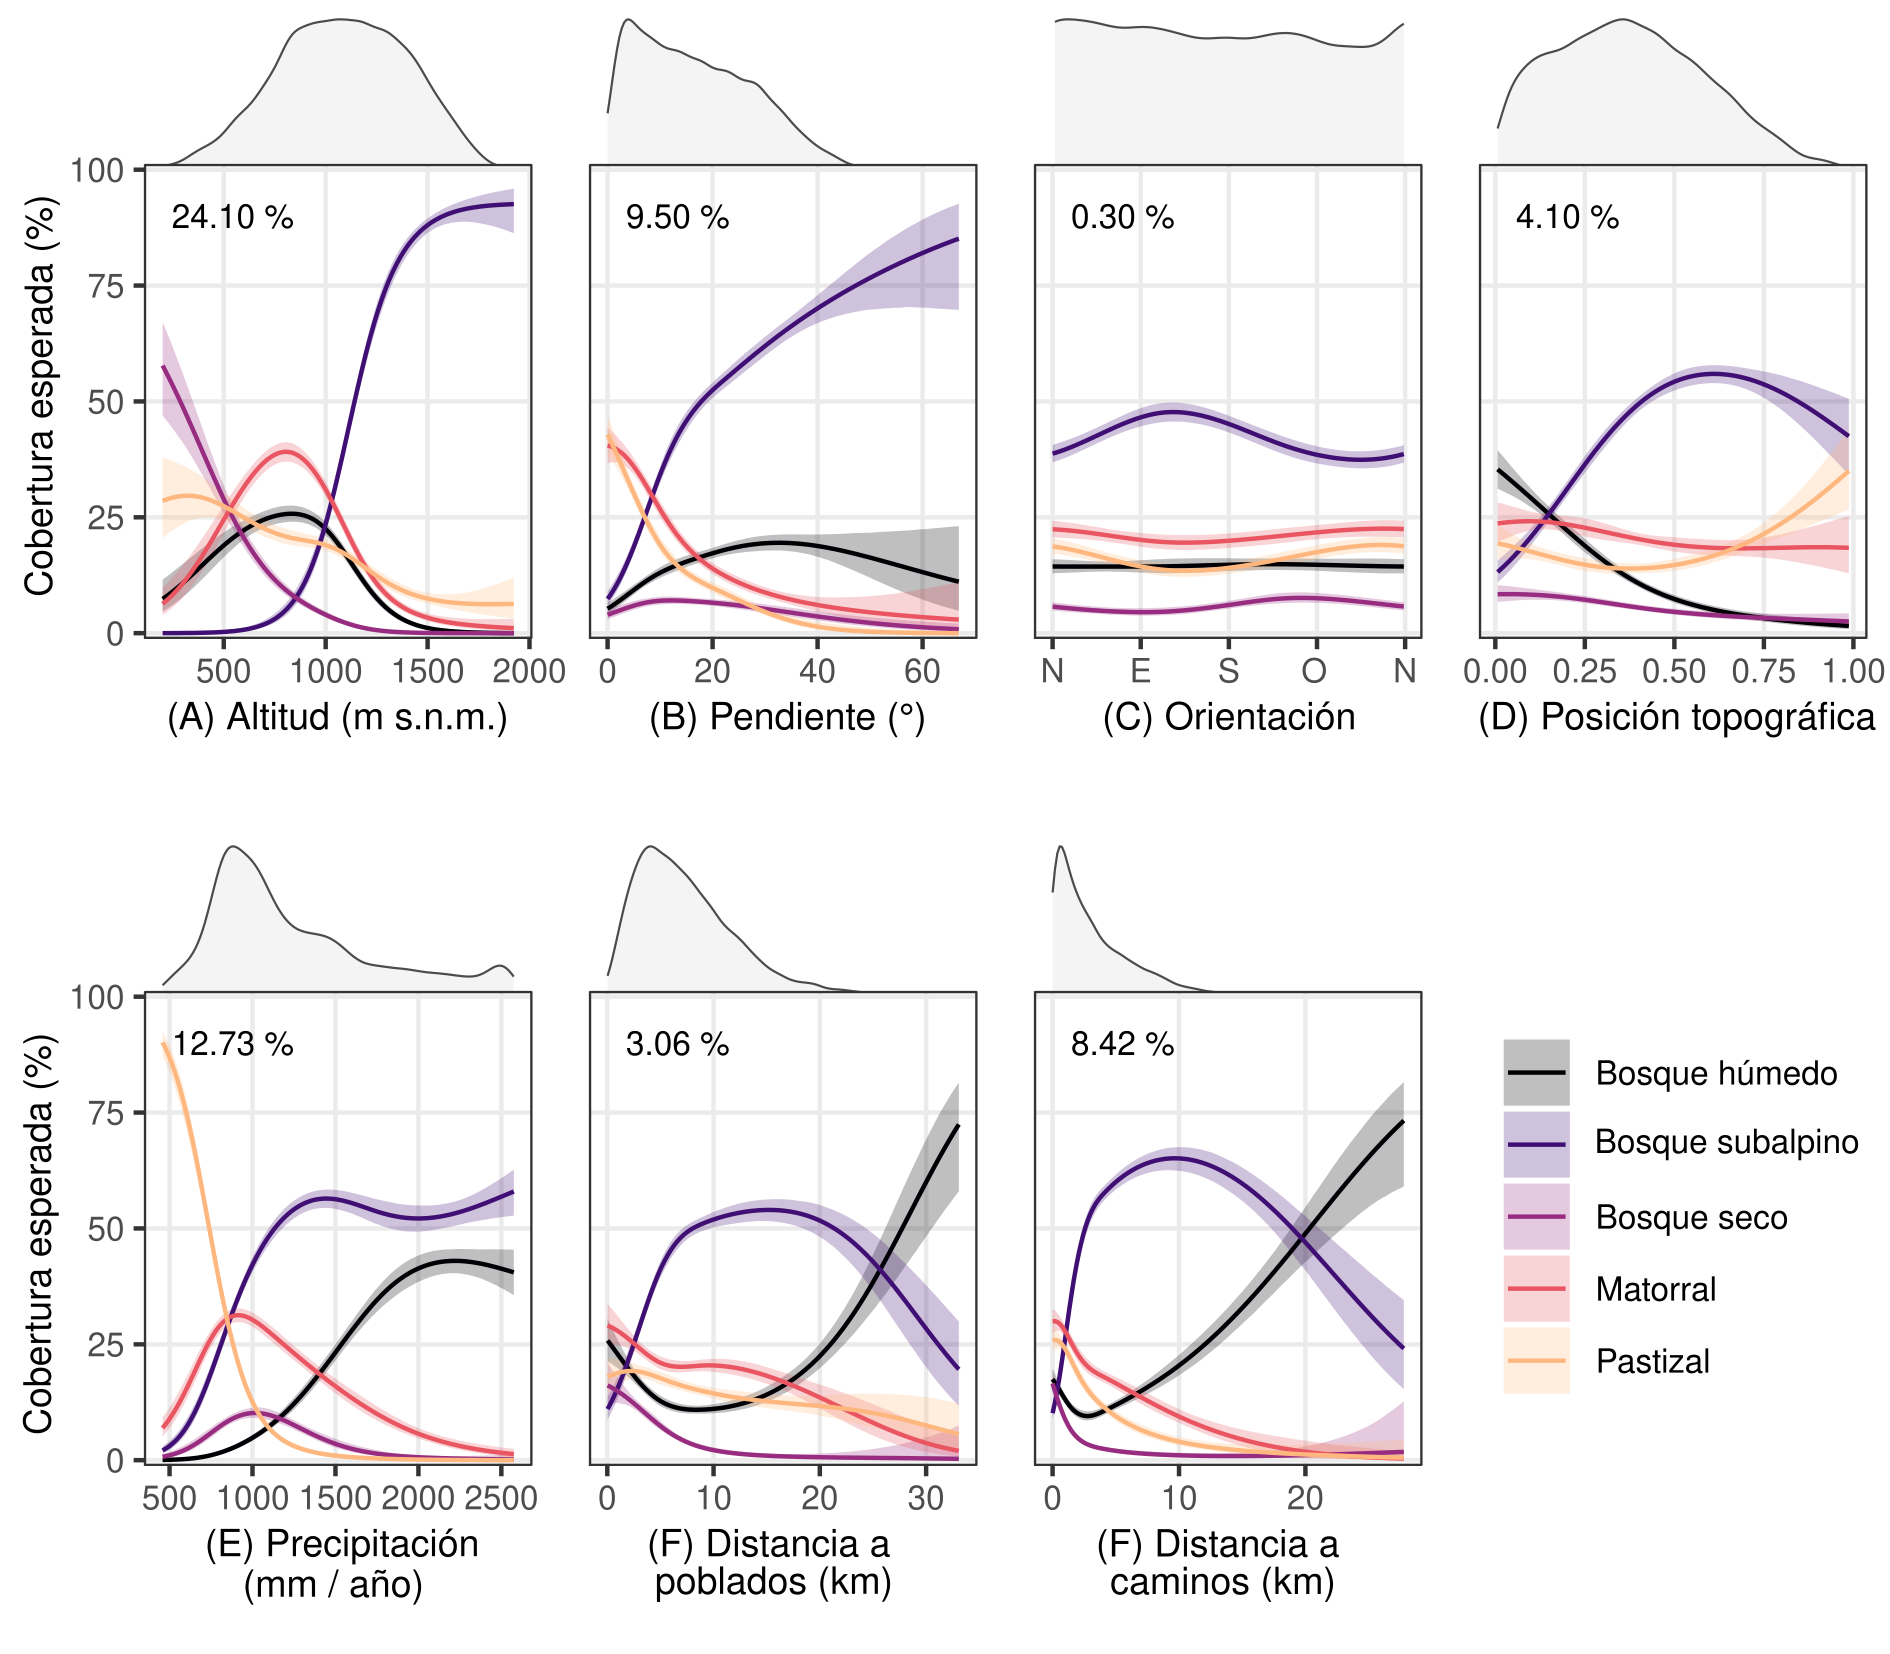
\includegraphics[width=16cm]{figuras/cap3/S01) vegetation_environment_marginal.png}
    \caption[Tipo de vegetación en función de variables ambientales, modelos univariados.]{Cobertura esperada (\%) de cada tipo de vegetación en función de las variables ambientales. Las líneas muestran la probabilidad estimada a partir de GAMs categóricos univariados con sus intervalos de confianza del 95 \%. Nótese que para cada valor de las predictoras todos los tipos suman 100 \%. Los números dentro de los paneles muestran el $\text{R}^2$ bayesiano de cada modelo, calculado como la media ponderada por abundancia del $\text{R}^2$ de cada tipo de vegetación, asumiendo una distribución Bernoulli de cada tipo. Las curvas grises arriba de los paneles muestran la distribución de cada variable predictora.} 
    \label{fig:cap3-S01}
\end{figure}


\begin{figure}
    \centering
    \rotatebox[origin=c]{90}{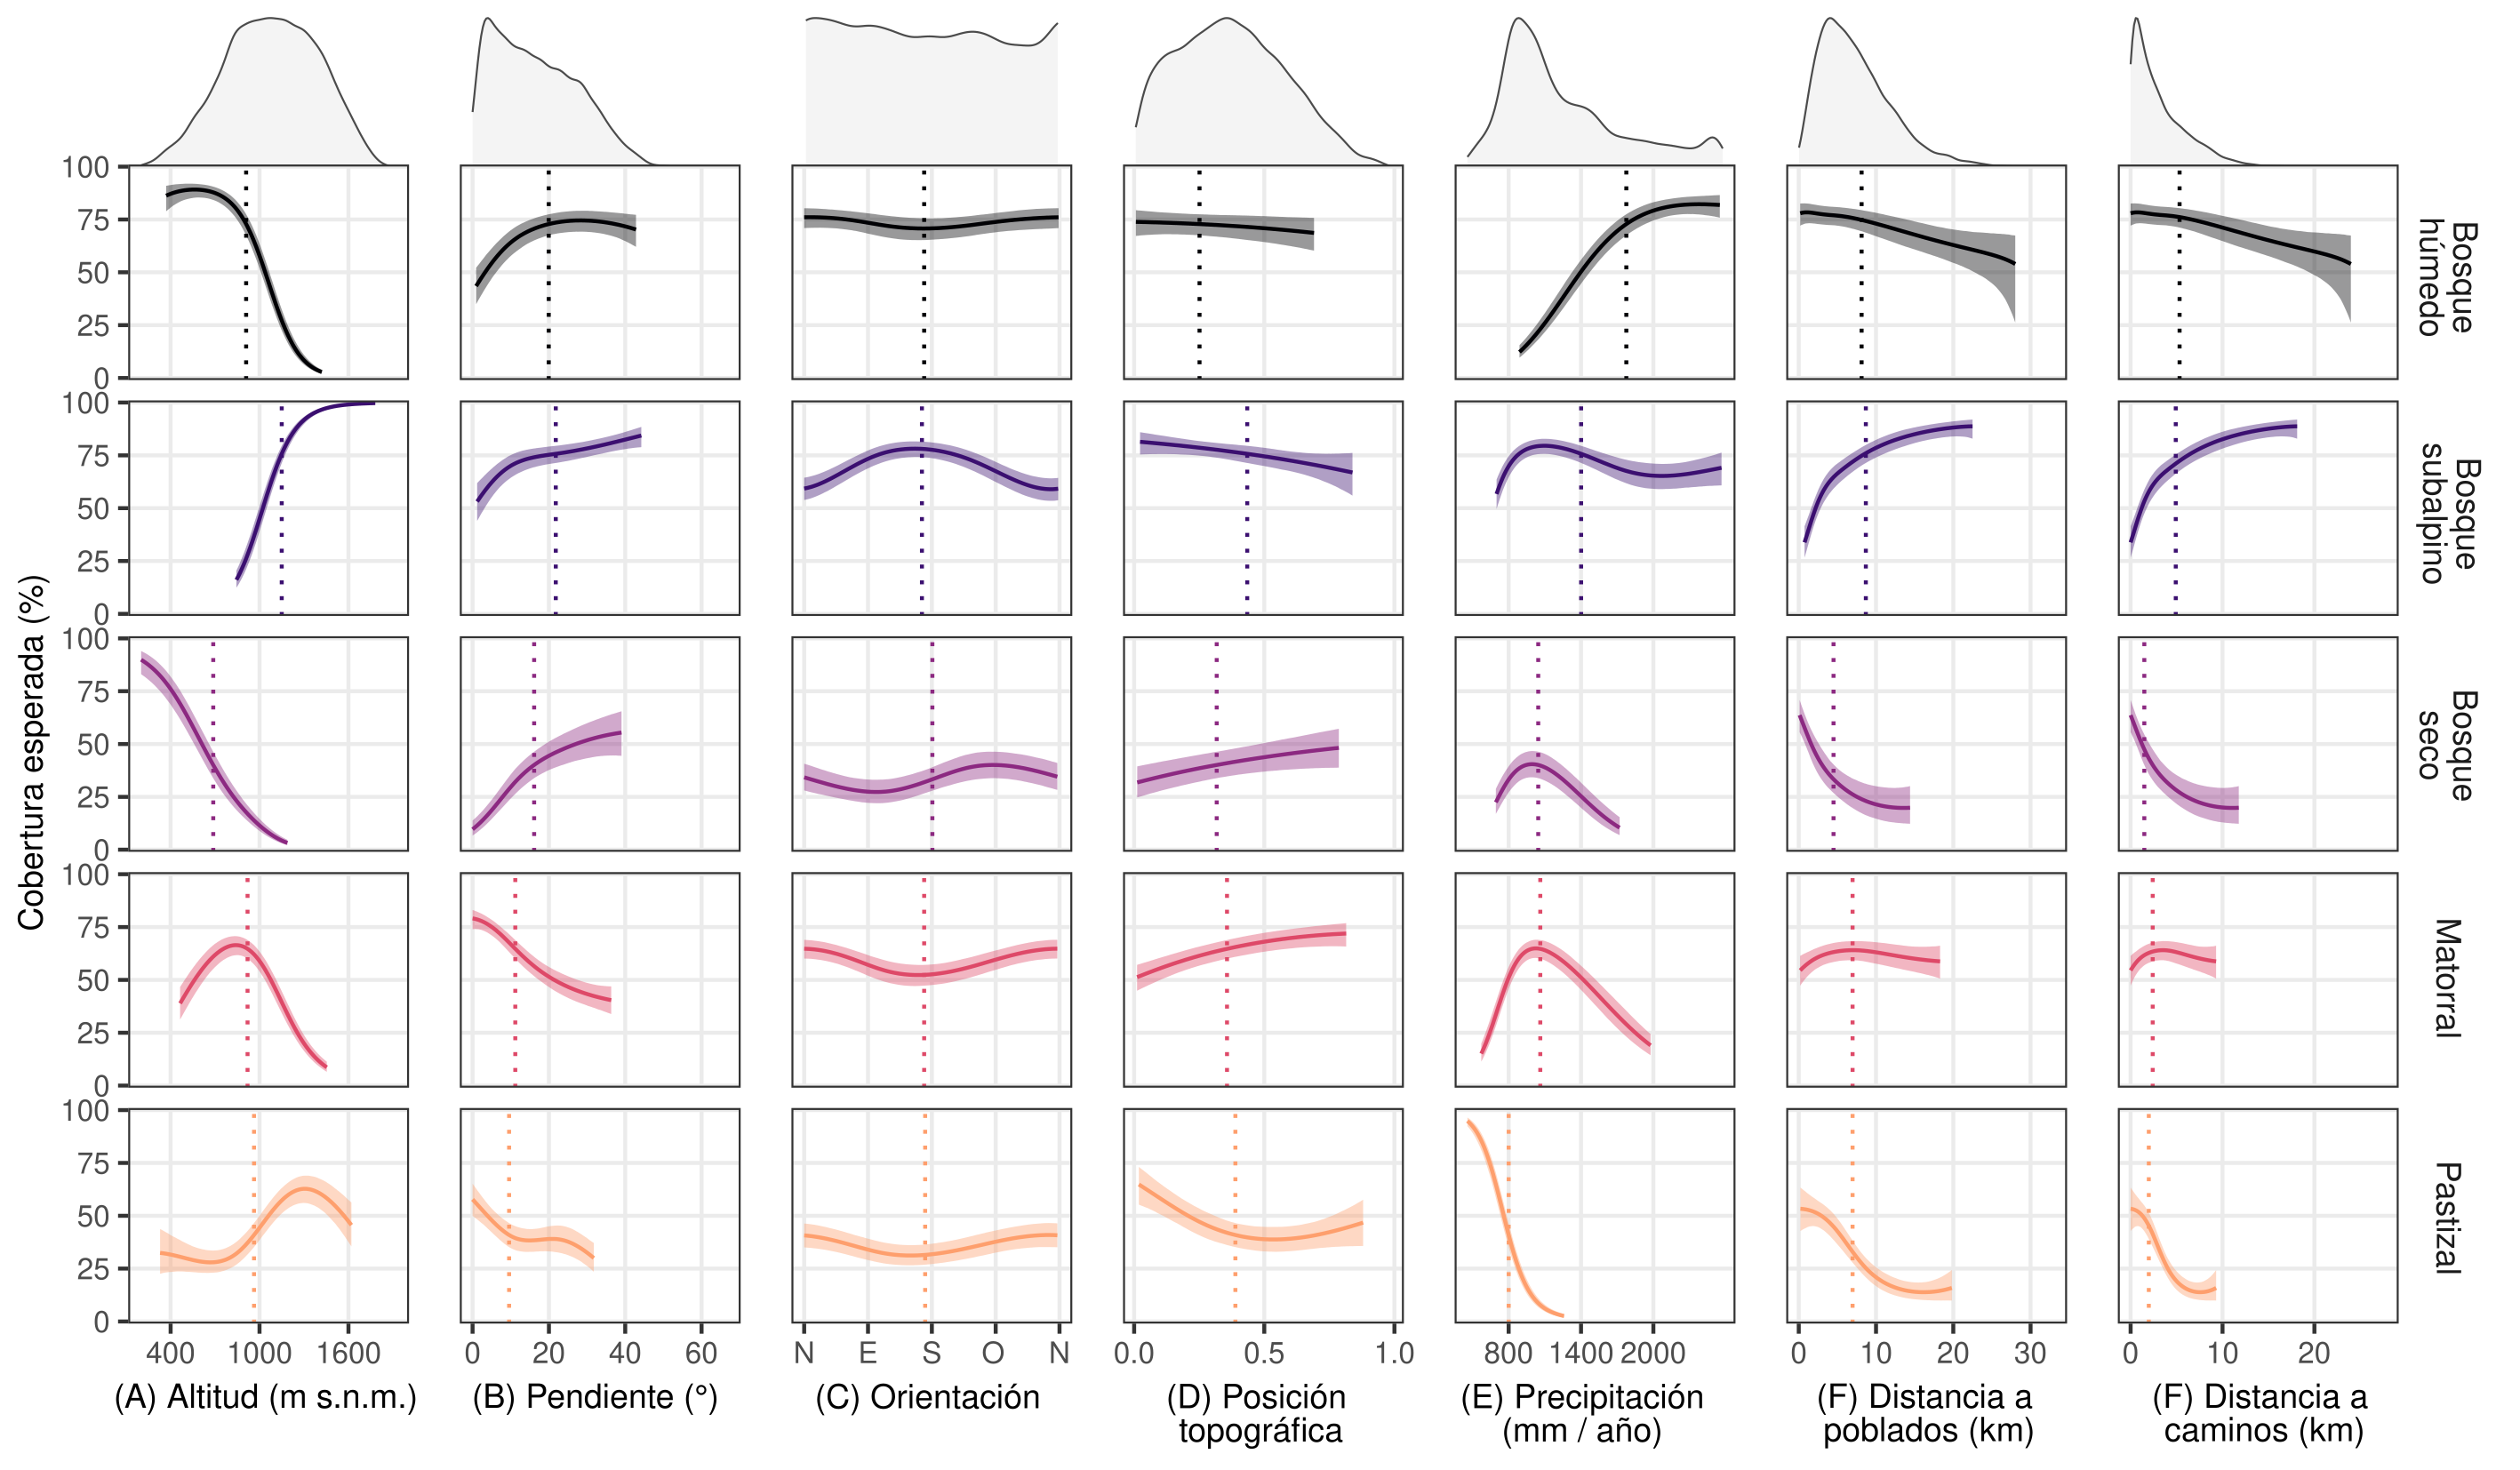
\includegraphics[width=0.95\textheight]{figuras/cap3/S02) vegetation_environment_conditional.png}}
    \caption[Tipo de vegetación en función de variables ambientales, modelo multivariado.]{(Leyenda en la página siguiente.)} 
    \label{fig:cap3-S02}
\end{figure}

% leyenda en la página siguiente
\begin{figure}[p]
  \contcaption{(en la página anterior). Cobertura esperada de cada tipo de vegetación en función de las variables ambientales, calculada a partir del GAM categórico de regresión múltiple. En cada panel se varía la predictora en el rango de cada tipo de vegetación, con el resto de las predictoras fijadas en la media correspondiente a cada tipo de vegetación (indicado con líneas verticales). En el caso del bosque subalpino, la altitud se fijó en 1150, en lugar de 1322 m s.n.m., para evitar que la cobertura esperada fuera cercana al 100 \%, ya que en este valor no se podían detectar efectos de otras predictoras. Las curvas grises arriba de los paneles muestran la distribución de cada variable predictora. Las predicciones abarcan el intervalo de mayor densidad del 98 \% de cada predictora en cada tipo de vegetación.} 
\end{figure}


\begin{table}
\caption[$\text{R}^2$ para los modelos de vegetación.]{$\text{R}^2$ (\%) para los modelos de tipo de vegetación, tanto univariado como multivariado (última inferior). El $\text{R}^2$ se calculó para cada tipo por separado como el $\text{R}^2$ bayesiano para una variable con distribución Bernoulli. En la figura~\ref{fig:cap3-S01} se muestra la media de $\text{R}^2$ ponderada por abundancia para cada modelo univariado. Las predicciones del modelo de regresión múltiple se muestran en la figura~\ref{fig:cap3-S02}.}
\label{tab:cap3-S01}
\resizebox{16cm}{!}{%
\begin{tabular}{l|ccccc}
\toprule
Variable & Bosque húmedo & Bosque subalpino & Bosque seco & Matorral & Pastizal \\
\midrule
Altitud & 7.16 & 46.11 & 13.98 & 10.79 & 2.75\\
Pendiente & 1.46 & 14.34 & 0.19 & 7.79 & 9.72\\
Orientación & 0.00 & 0.53 & 0.21 & 0.07 & 0.28\\
Posición topográfica & 6.76 & 6.95 & 0.53 & 0.28 & 0.55\\
Precipitación & 17.61 & 8.84 & 2.30 & 5.86 & 31.31\\
Distancia a poblados & 2.44 & 5.41 & 3.41 & 0.69 & 0.44\\
Distancia a caminos & 4.20 & 14.44 & 4.18 & 3.28 & 4.73\\
\midrule
Regresión múltiple & 43.04 & 56.77 & 27.72 & 24.87 & 40.67\\
\bottomrule
\end{tabular}
}
\end{table}

Estos patrones indican que a pesar de que las variables ambientales están asociadas al tipo de vegetación, la relación no es demasiado estrecha, lo que permite separar aproximadamente los efectos del tipo de vegetación y las variables ambientales sobre el fuego. Esto es posible por dos razones. La primera es que con un considerable solapamiento entre tipos de vegetación a lo largo de gradientes ambientales podemos comparar la probabilidad de quema estimada entre tipos de vegetación bajo las mismas condiciones ambientales, representando efectos más puros de la vegetación sobre el fuego. Esto permite comparar cómo cambia el patrón de probabilidad de quema entre tipos de vegetación si se controlan o no las variables ambientales (Fig.~\ref{fig:cap3-06}C vs. \ref{fig:cap3-06}A, respectivamente). La segunda razón es la gran variación ambiental dentro de los tipos de vegetación (ver densidades rosas en Fig.~\ref{fig:cap3-04} y \ref{fig:cap3-05}, filas 2 a 6), que permiten estimar el efecto de las variables ambientales dentro de los tipos de vegetación, para compararlo con su efecto global, que ignora el tipo de vegetación (primera fila en Fig.~\ref{fig:cap3-04} y \ref{fig:cap3-05}). Estos aspectos de los datos están representados por los modelos que predicen el tipo de vegetación (Fig.~\ref{fig:cap3-S01} y \ref{fig:cap3-S02}) y por la distribución de las variables ambientales dentro de los tipos de vegetación (Fig.~\ref{fig:cap3-04} y \ref{fig:cap3-05}, filas 2 a 6). Pero a su vez, puede notarse de forma más compacta identificando los tipos de vegetación en un ordenamiento de los puntos muestreados según las variables ambientales (Fig.~\ref{fig:cap3-S03}). Las regiones de mayor densidad para las coordenadas del Análisis de Componentes Principales por tipo de vegetación muestran un solapamiento considerable, y también reflejan una notable variación ambiental dentro de cada tipo.

\begin{figure}[htbp]
    \centering
    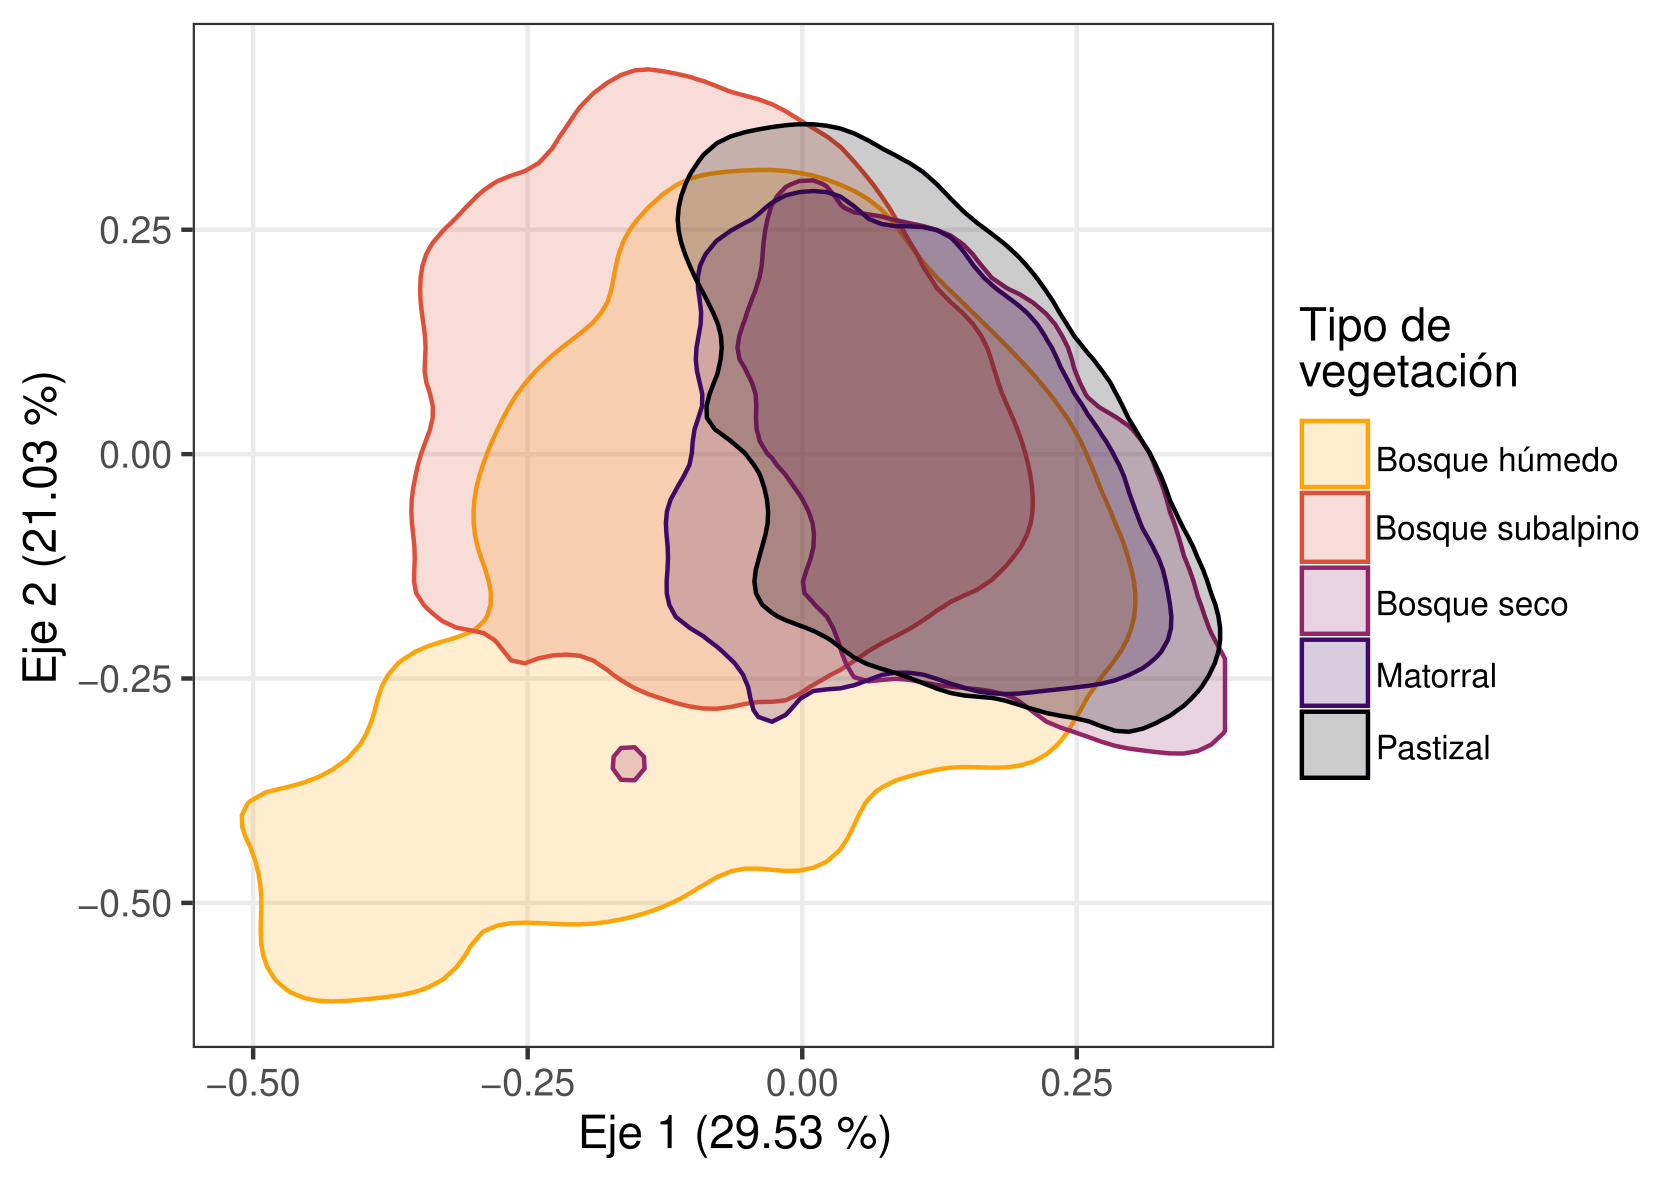
\includegraphics[width=14cm]{figuras/cap3/S03) ordination.png}
    \caption[Ubicación de tipos de vegetación en un ordenamiento basado en variables ambientales.]{Primeros dos ejes de un Análisis de Componentes Principales (ACP) realizado con las 7 predictoras ambientales: altitud, pendiente, orientación [transformado a su componente norte como cos(orientación)], posición topográfica, precipitación, distancia a poblados y distancia a caminos. Como teníamos demasiados puntos de datos para visualizarlos correctamente (N = 8018), sólo mostramos las regiones de mayor densidad del 90 \% para las coordenadas del ACP de cada tipo de vegetación. Los datos se agruparon por tipo de vegetación luego de correr el ACP. Los porcentajes indican la parte de la varianza explicada por cada eje.} 
    \label{fig:cap3-S03}
\end{figure}

\begin{figure}[htbp]
    \centering
    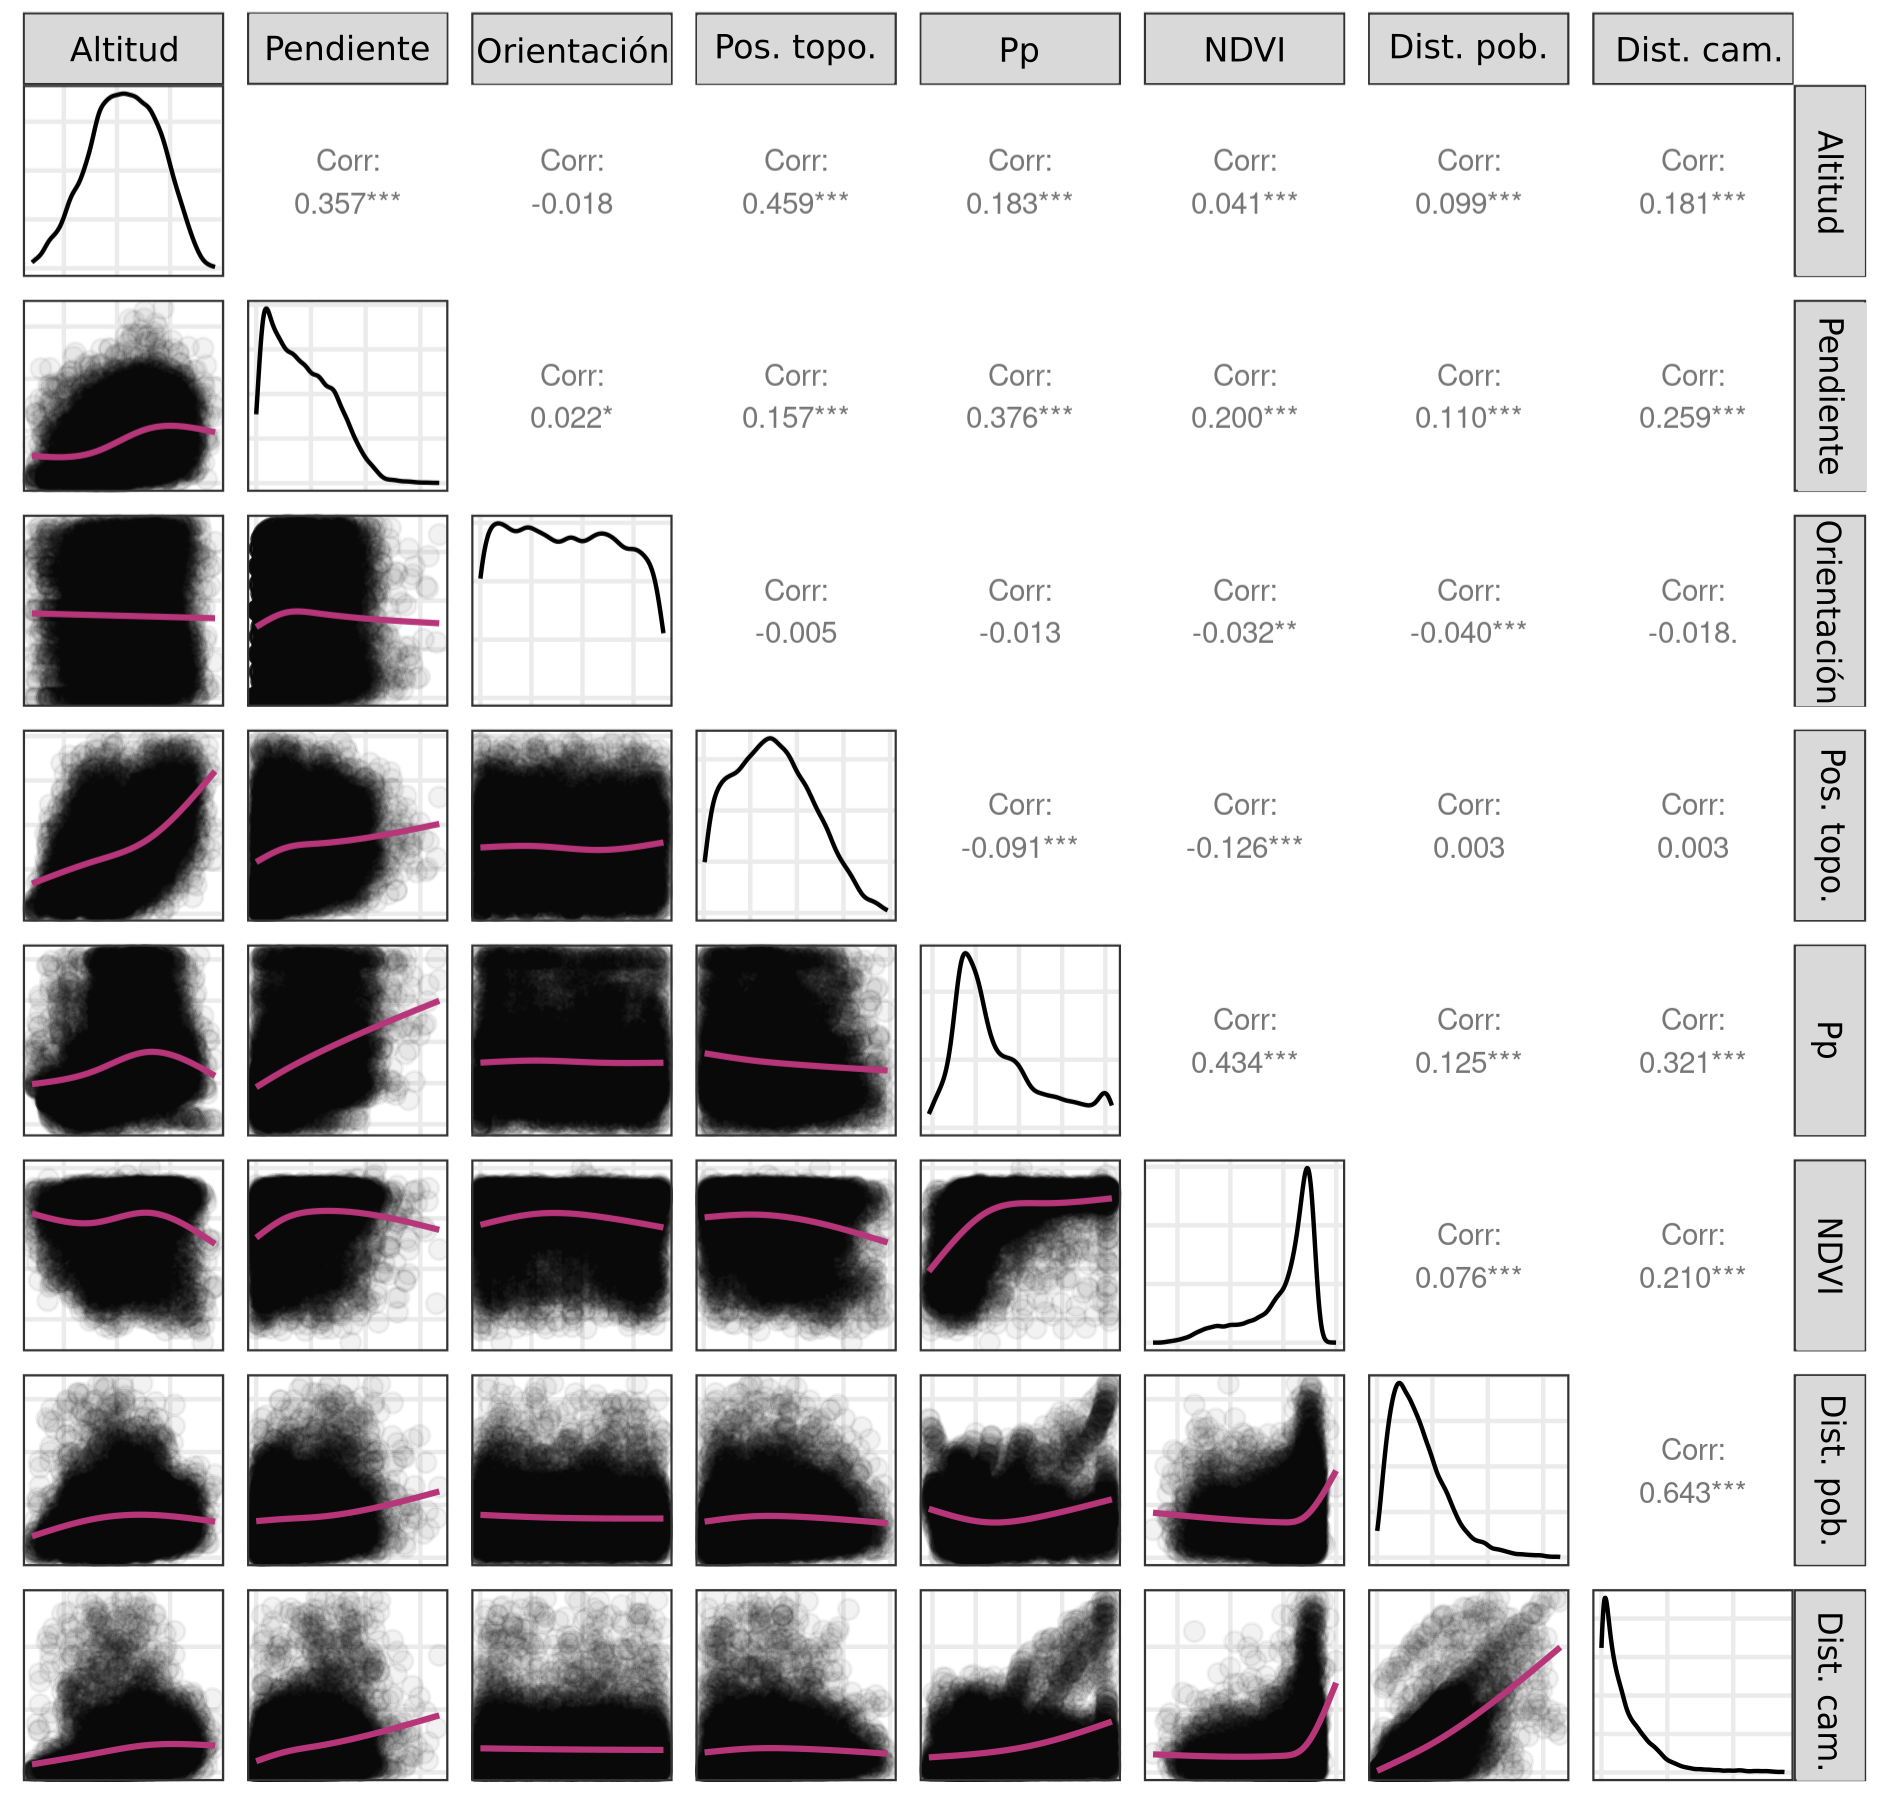
\includegraphics[width=16cm]{figuras/cap3/S04) correlations_env.png}
    \caption[Correlación entre predictoras ambientales.]{Diagramas de dispersión de todas las predictoras de probabilidad de quema, utilizando los 8228 puntos muestreados en el área quemable. Las líneas muestran el ajuste de un GAM con \textit{splines} cúbicas de tres funciones base (\texttt{k = 4} en \texttt{mgcv}), asumiendo una distribución normal de la respuesta. En los paneles diagonales se muestra la distribución de cada variable, y los números de los paneles superiores muestran el coeficiente de correlación de Pearson. Abreviaturas: Pos. topo: posición topográfica; Pp: precipitación; Dist. pob.: distancia a poblados; Dist. cam.: distancia a caminos.} 
    \label{fig:cap3-S04}
\end{figure}

\FloatBarrier

\section{Mapeo de incendios}\label{append:mapeo}

El procedimiento de mapeo fue semiautomático: en primer lugar, produjimos polígonos de áreas quemadas con un enfoque automático en Google Earth Engine \citep{gorelick_google_2017} utilizando índices de quema y de vegetación (NDVI: Índice de Vegetación de Diferencia Normalizada y NBR: Razón de Quema Normalizado), y luego editamos manualmente los polígonos de incendios para corregir errores (Fig.~\ref{fig:cap3-S05}). El enfoque automático resultó confiable para detectar la ubicación de los incendios, pero como la señal de quema (reducciones de NBR y NDVI) permanece al menos un año después del incendio, muchos incendios o partes de ellos se asignaban incorrectamente a años adyacentes. Además, las zonas quemadas muestran propiedades espectrales similares a las zonas afectadas por otros disturbios, como talas y defoliaciones por insectos, lo que hace que el procedimiento automático genere cierto grado de error de comisión. La revisión manual permitió superar estos problemas. La base de datos está disponible públicamente en GitHub (\url{https://github.com/barberaivan/patagonian_fires.git}).

Realizamos el mapeo de incendios en pasos anuales, pero como la mayor parte de ellos ocurren entre diciembre y marzo en nuestra área de estudio, consideramos los años corriendo de julio a junio, etiquetándolos con el año del mes final para simplificar. Por ejemplo, un incendio ocurrido en octubre de 1998 se asigna al año de fuego 1999.

\begin{figure}[htbp]
    \centering
    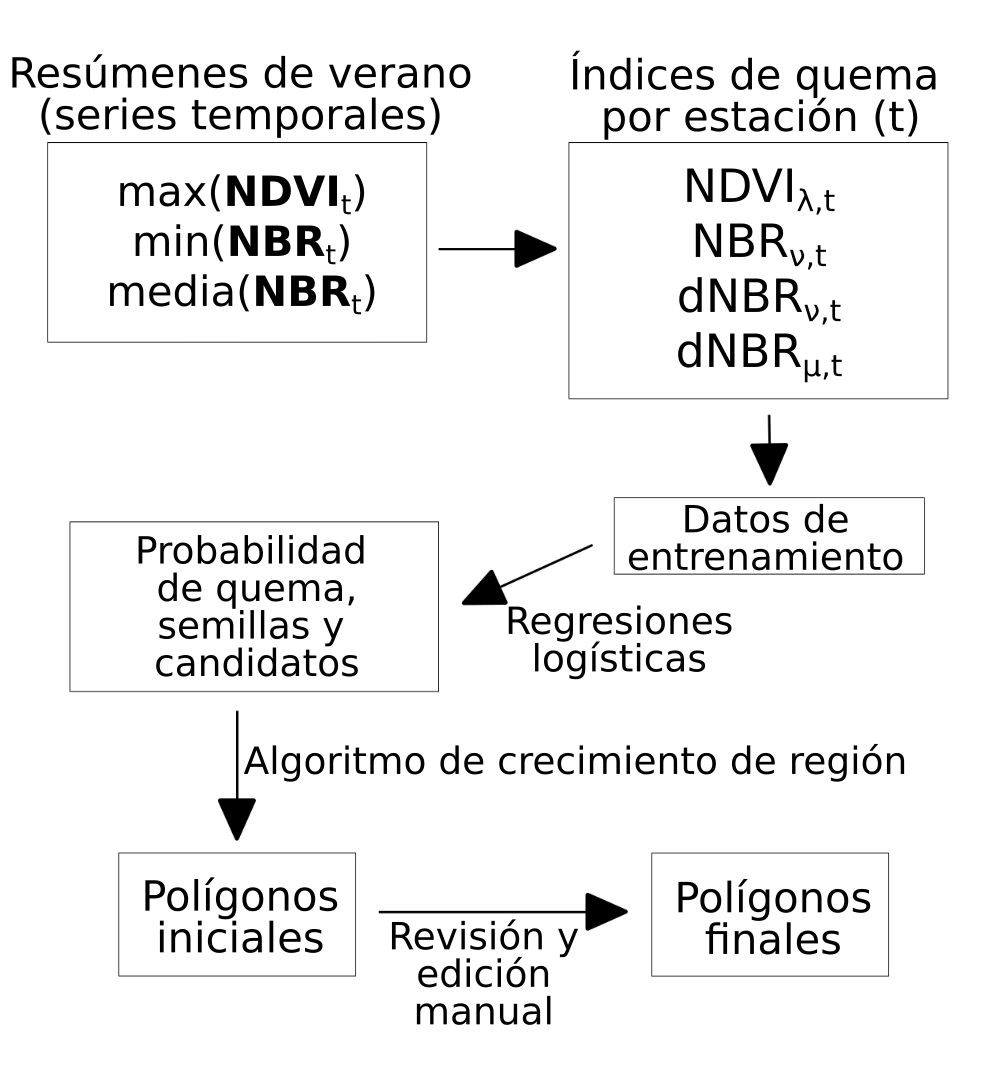
\includegraphics[width=9cm]{figuras/cap3/S05) mapping_algorithm.png}
    \caption[Algoritmo de mapeo de incendios.]{Esquema del algoritmo de mapeo de incendios. La mayor parte del procedimiento se llevó a cabo en Google Earth Engine \citep{gorelick_google_2017}, mientras que las regresiones logísticas se ajustaron en R \citep{R}, y para la revisión y edición manual utilizamos ambos software combinados con QGIS \citep{qgis326}. Los índices de vegetación brutos utilizados fueron el NDVI y el NBR; los índices de quema por estación se definen en la Ecuación~\ref{eq:cap3-burnindex}. El sufijo $t$ indica cada año, incluyendo imágenes sólo de diciembre a abril y tomando la etiqueta del año final.} 
    \label{fig:cap3-S05}
\end{figure}

\subsection{Fase automática}

La etapa de mapeo automático fue similar a la descrita por \citet{long2019}, basada en un algoritmo de crecimiento de región: para cada año desde 1999 hasta 2022 (incluido) definimos por separado los píxeles con alta probabilidad de ser quemados, llamados semillas, y los píxeles con probabilidad baja o media, llamados candidatos. El algoritmo de crecimiento de región genera grupos de píxeles quemados a partir de las semillas, se y extiende hasta incluir todos los píxeles candidatos vecinos (8 píxeles) (algoritmo SNIC en Google Earth Engine; \citealt{AchantaSNIC}). La probabilidad de quema a nivel de píxel utilizada para definir semillas y candidatos se definió mediante tres modelos de regresión logística, utilizando índices basados en NDVI y NBR como predictoras (Fig.~\ref{fig:cap3-S06}A). Para cada año, calculamos el NDVI y el NBR a partir de todas las imágenes Landsat disponibles (producto de \textit{Surface Reflectance}, Colecciones 1 y 2) que intersecaban el área de estudio, tomadas entre diciembre y abril (incluidos), ya que este periodo tiene baja nubosidad. A partir de estas variables, calculamos cuatro índices derivados por año ($t$):

\begin{equation}
\begin{aligned}
    \text{NDVI}_{\lambda,t} &= \text{max}(\{\textbf{NDVI}_t, \textbf{NDVI}_{t-1}\}) \\  
    \text{dNBR}_{\mu,t} &= \text{media}(\textbf{NBR}_{t-1}) - \text{media}(\textbf{NBR}_{t+1})  \\
    \text{dNBR}_{\nu,t} &= \text{min}(\textbf{NBR}_{t-1}) - \text{min}(\textbf{NBR}_{t}) \\
    \text{NBR}_{\nu,t} &= \text{min}(\textbf{NBR}_t),
\end{aligned}
\label{eq:cap3-burnindex}
\end{equation}

\noindent y el máximo de los promedios de NDVI por año (verano):

\[
\text{NDVI}_{\lambda,\mu} = \text{max}[\{\text{media}(\textbf{NDVI}_{1999}), ..., \text{media}(\textbf{NDVI}_{2022})\}].
\]

\noindent Las variables en negrita representan vectores con todos los valores disponibles de los índices espectrales correspondientes entre diciembre y abril del año $t$, para cada píxel (ejemplo: para 1999 se utilizan imágenes de diciembre de 1998 a abril de 1999). A partir de los cuatro índices dinámicos (con el sufijo $t$) ajustamos tres regresiones logísticas para modelar la probabilidad de quema a nivel de píxel, definidas de la siguiente manera: 

\begin{equation}
\begin{aligned}
\text{logit}(p_{1,t}) &=  \alpha_1 + \beta_1 \ \text{dNBR}_{\mu,t}  +  \gamma_1 \ \text{NDVI}_{\lambda,t} + \delta_1 \ \text{dNBR}_{\mu,t} \ \text{NDVI}_{\lambda,t} \\
\text{logit}(p_{2,t}) &=  \alpha_2 + \beta_2 \ \text{dNBR}_{\nu,t}  +  \gamma_2 \ \text{NDVI}_{\lambda,t} + \delta_2 \ \text{dNBR}_{\nu,t} \ \text{NDVI}_{\lambda,t} \\
\text{logit}(p_{3,t}) &=  \alpha_3 + \beta_3 \ \text{NBR}_{\nu,t}  +  \gamma_3 \ \text{NDVI}_{\lambda,t} + \delta_3 \ \text{NBR}_{\nu,t} \ \text{NDVI}_{\lambda,t}.
\end{aligned}
\label{eq:cap3-burnmap}
\end{equation}

Ajustamos los modelos utilizando píxeles seleccionados en incendios conocidos y sus alrededores. Elegimos cinco incendios grandes bien documentados y seleccionamos visualmente aproximadamente 300 píxeles quemados y unos 300 no quemados por incendio, basándonos en la composición RGB de las imágenes Landsat poco después del fuego. Aprendimos a distinguir entre píxeles quemados y no quemados basándonos en el color de la imagen, evaluando si la serie temporal de NBR mostraba un descenso, e inspeccionando las imágenes de Google Earth en las que las zonas quemadas eran evidentes. El $\text{NDVI}_{\lambda,t}$ se incluyó para permitir que los umbrales basados en índices basados en NBR variaran en función de la productividad del píxel, ya que las áreas de baja productividad, como los pastizales, presentan una menor disminución de NBR cuando se queman comparado con las áreas de alta productividad, como los bosques (Fig.~\ref{fig:cap3-S06}A). Esta estrategia es similar al uso de índices de quema relativizados, como RdNBR \citep{miller2007rdNBR}, pero análisis exploratorios sugirieron que nuestro enfoque sería más preciso. También probamos Random Forests y Support Vector Machines, incluyendo como predictoras las bandas Landsat sin procesar y varios índices de vegetación. Como no encontramos mejoras en la precisión, optamos por los métodos de regresión más sencillos e interpretables.

Definimos las semillas como píxeles con probabilidad de quema $\ge 0.98$ para los tres modelos que también mostraban alta productividad ($\text{NDVI}_{\lambda,\mu} \ge 0.7$) o baja altitud ($<$ 1300 m s.n.m.). Con estas restricciones adicionales se evitaron falsos positivos que aparecían en zonas altoandinas, frecuentemente cubiertas de nieve. Los candidatos se definieron por separado en función de la productividad de los píxeles:

\begin{enumerate}
    \item $p_1 \ge 0.20$ si $\text{NDVI}_{\lambda,t} > 0.5$, y
    \item $\{p_2, p_3\} \ge 0.25$ si $\text{NDVI}_{\lambda,t} \le 0.7$. 
\end{enumerate}    

\noindent De este modo, los índices utilizados para definir la probabilidad de quema de los píxeles de baja productividad ($\text{NDVI}_{\lambda,t} \le 0.7$) no utilizan el NBR del año siguiente ($t+1$), lo que resultaba conveniente porque los pastizales se recuperan rápidamente, por lo que $p_1$ no detecta correctamente los pastizales quemados. Por el contrario, las zonas boscosas $\text{NDVI}_{\lambda,t} > 0.5$ muestran una disminución prolongada del NBR cuando se queman, por lo que el uso de $p_1$ es mejor para clasificar esos píxeles. La figura~\ref{fig:cap3-S06}B muestra las tasas de error por comisión y omisión de cada modelo.
A los polígonos de incendios del mismo año se les asignó el mismo ID de incendio si estaban separados por menos de 85 m (más cerca que dos píxeles diagonales de 30 m).

\begin{figure}[htbp]
    \centering
    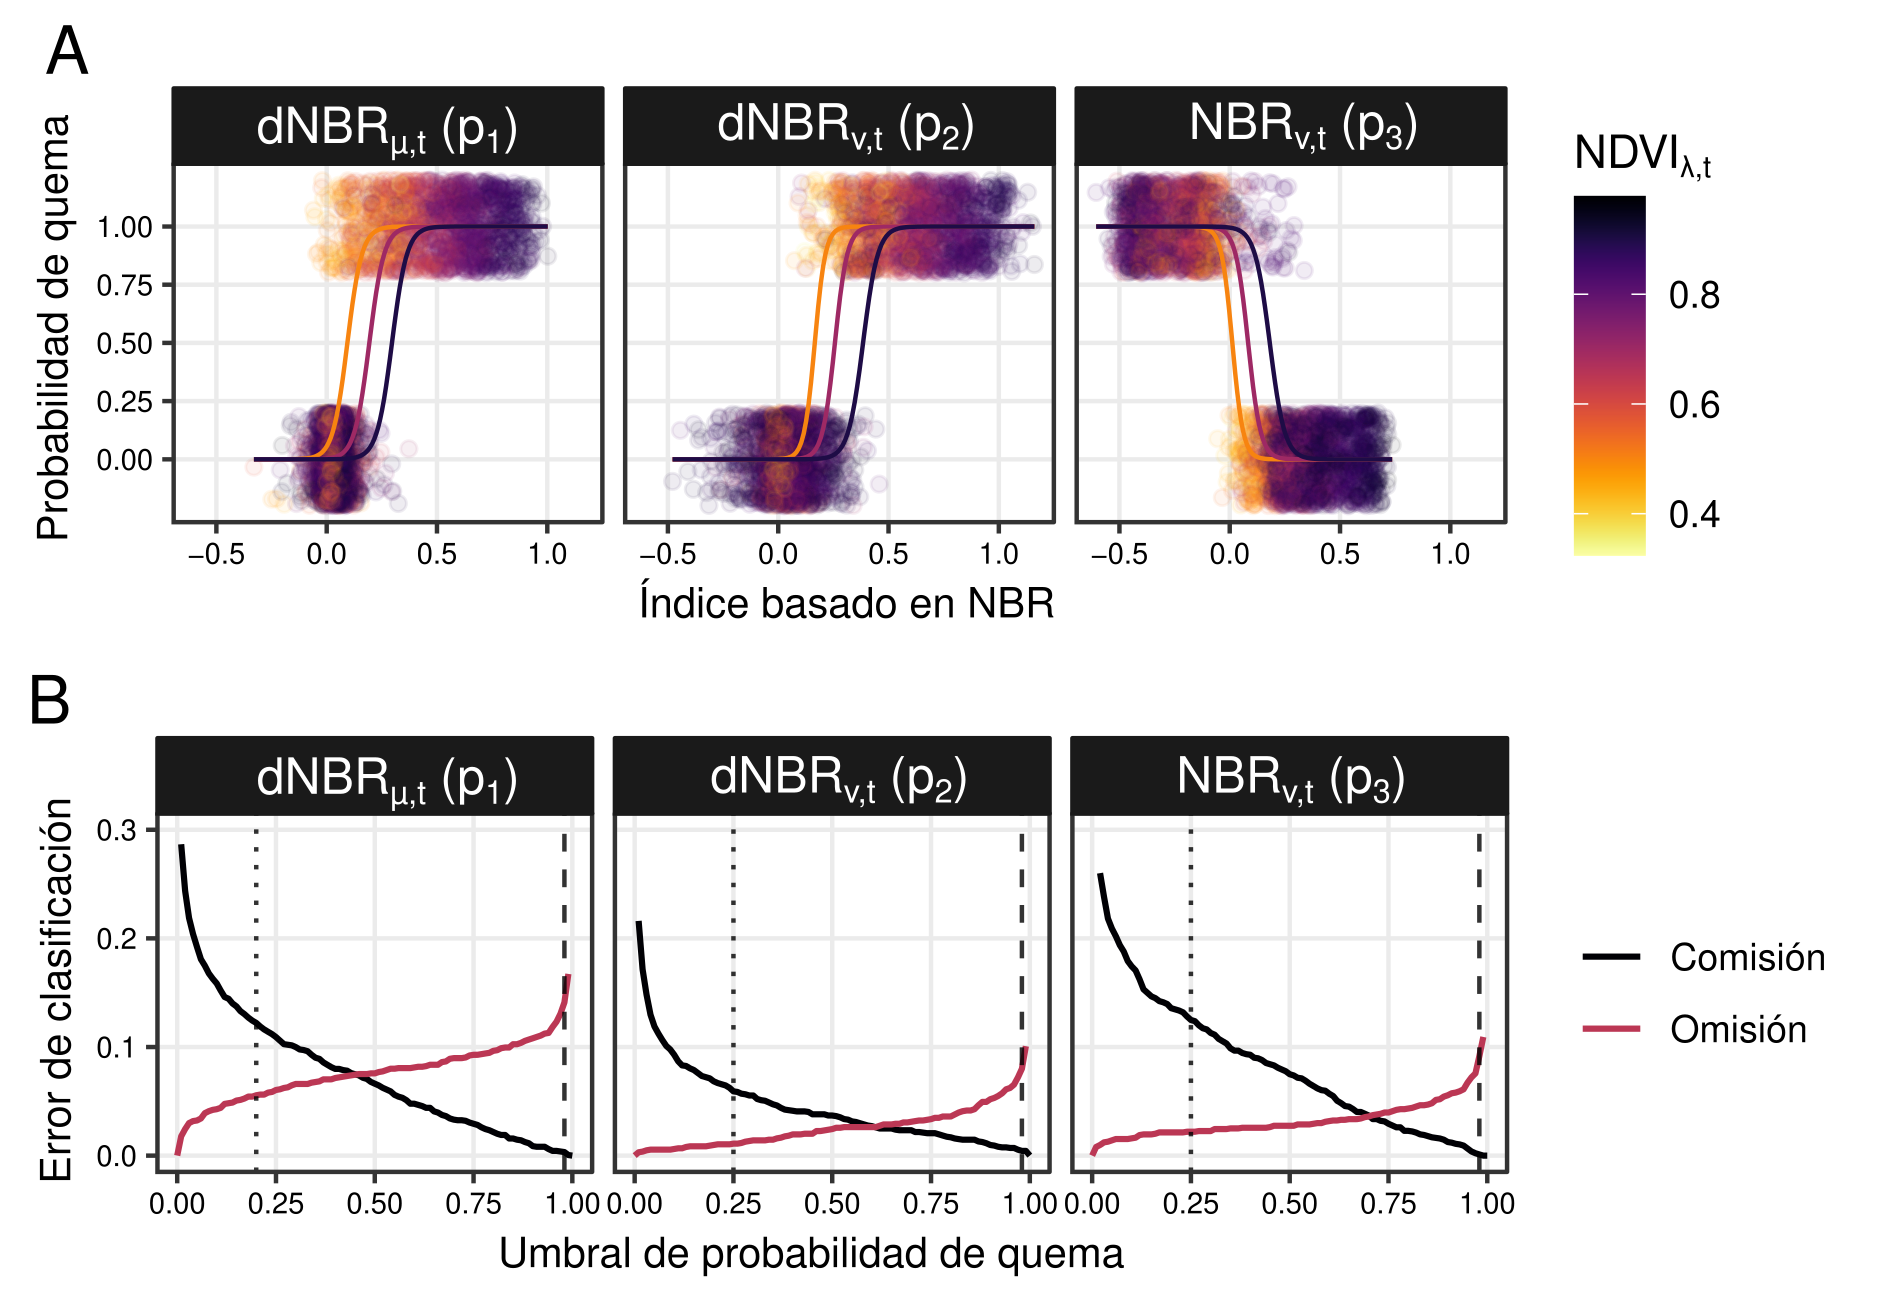
\includegraphics[width=16cm]{figuras/cap3/S06) mapping_error.png}
    \caption[Modelos de probabilidad de quema utilizados en el mapeo de incendios.]{(A) Funciones de probabilidad de quema utilizadas para clasificar los píxeles quemados, definidas por índices espectrales calculados a partir de imágenes Landsat (ver Ecuación~\ref{eq:cap3-burnmap}). Las líneas muestran la probabilidad de quema predicha para cada modelo en diferentes valores de $\text{NDVI}_{\lambda,t}$ (0.5, 0.7 y 0.9). Los puntos muestran los datos de entrenamiento (quemado = 1, no quemado = 0) con un \textit{jitter} en el eje $y$ para mejorar la visibilidad. Los modelos se entrenaron con 3480 píxeles pertenecientes a cinco incendios. (B) Tasas de error de comisión y omisión en función del umbral de probabilidad de quema, calculado con una validación cruzada tomando los datos de cada incendio como particiones. El error de comisión es la proporción de píxeles no quemados en el conjunto de prueba clasificados como quemados, y el error de omisión es la proporción de píxeles quemados clasificados como no quemados. Las líneas verticales discontinuas muestran los umbrales de probabilidad de quema utilizados para los candidatos (0.20 o 0.25, según el modelo) y las líneas discontinuas muestran el umbral utilizado para las semillas (0.98) en el algoritmo de crecimiento de región. Con estos umbrales se obtuvo un error de omisión bajo para los candidatos y un error de comisión bajo para las semillas.} 
    \label{fig:cap3-S06}
\end{figure}

\subsection{Fase manual}\label{append:mapeo-manual}

Revisamos todos los polígonos de incendios $\ge$ 10 ha y eliminamos aquellos confundidos con urbanización, zonas cultivadas, deforestación, nieve o hielo, zonas inundadas o incendios ocurridos en años adyacentes. Además, unimos (dividimos) polígonos de incendios cercanos pertenecientes al mismo (distinto) incendio, basándonos en el conocimiento local o en las fechas de quema. 
Algunos polígonos que presentaban un mapeo deficiente, detectado visualizando la serie temporal de NBR, fueron editados en base a la diferencia en NBR de fechas pre y post incentdio.
En 1999 se disponía de pocas imágenes en la zona de estudio, por lo que algunos incendios no pudieron mapearse con la precisión deseada, por lo que incluimos en nuestra base de datos tres incendios de 1999 mapeados por la Administración de Parques Nacionales de Argentina \citep{mermoz_deteccion_2002}.

\subsection{Definición de la fecha del incendio}\label{append:fire-dating}

Algunos incendios estaban bien documentados, y la fecha de inicio se obtuvo de instituciones de gestión de incendios o de noticias. Si se conocía el periodo en el que el fuego quemó la mayor área, la fecha del incendio se definía como la fecha central del periodo. Si no se disponía del periodo, se fijaba la fecha de inicio. En el caso de los grandes incendios, complementamos esta información con el producto diario de área quemada de MODIS (MCD64A1) y los puntos calientes (MCD14DL), que ayudaron a definir el periodo en el que ardió la mayor parte de la superficie. Para los incendios de los que no se disponía de información y que no fueron detectados por MODIS, ya sea porque ocurrieron antes de 2001 o porque eran demasiado pequeños, definimos la fecha del incendio basándonos en las series temporales de NBR calculadas a partir de todas las imágenes Landsat disponibles. Inspeccionamos visualmente las series temporales dentro de los tres años anteriores y posteriores al supuesto año de quema para detectar una caída abrupta del NBR relacionada con el fuego. La fecha del incendio se definió como la fecha central entre el último día en que el NBR fue alto antes de la caída (más un día) y el primer día después de la caída en que el NBR fue bajo.

\subsection{Evaluación del error de mapeo}\label{append:mapeo-error}

Para cuantificar el error del procedimiento completo (automático + manual) evaluamos 22 incendios que podían identificarse claramente en Google Earth. Para cada incendio seleccionamos visualmente puntos quemados y no quemados utilizando Google Earth, y luego evaluamos si estaban dentro o fuera de su correspondiente polígono. El número de puntos tomados para cada incendio varió entre 28 y 289 (considerando por separado los quemados y los no quemados), dependiendo del tamaño del incendio y de la disponibilidad de imágenes claras en Google Earth para identificarlos correctamente (Tabla~\ref{tab:cap3-S02}). Para estimar el error medio de comisión y omisión entre incendios a partir de los conteos de puntos clasificados incorrectamente sobre el total en cada uno de los 22 conjuntos de datos de prueba, ajustamos un modelo Beta-Binomial para cada tipo de error. Este modelo estima la probabilidad de error en cada incendio como un efecto aleatorio, que sigue una distribución Beta, cuya media estimada representa el error medio entre incendios. El error de comisión medio fue del 0.64 \% (intervalo de confianza del 95 \%, IC = [0.32 \%; 1.30 \%]), y el error de omisión fue del 3.36 \% (IC del 95 \% = [2.02 \%; 5.52 \%]). La Tabla~\ref{tab:cap3-S02} muestra la tasa de error y la cantidad de puntos por fuego. La precisión se estimó de la misma manera, en un 98.06 \% (95 \% CI = [96.92 \%; 98.78 \%]).

\begin{table}[h!]
\centering
\caption[Precisión del mapeo de incendios.]{Error de omisión y comisión y precisión global del procedimiento de mapeo de incendios para 22 incendios. Los números entre paréntesis muestran la cantidad de puntos clasificados como no quemados que en realidad estaban quemados sobre el número de puntos de prueba quemados (omisión), la cantidad de puntos clasificados como quemados que en realidad no estaban quemados sobre el número de puntos de prueba no quemados (comisión), y el número de puntos -quemados o no quemados- clasificados correctamente sobre el total (precisión).}
\label{tab:cap3-S02}
\resizebox{16cm}{!}{%
\begin{tabular}{c|ccc}
\toprule
Incendio (ID) & Error de omisión (\%) & Error de comisión (\%) & Precisión (\%) \\
\midrule
2008\_1379405717 & 0 (0/133) & 0 (0/116) & 100 (249/249) \\
2008\_3 & 0 (0/59) & 1.32 (1/76) & 99.26 (134/135) \\
2008\_5 & 0 (0/62) & 0 (0/179) & 100 (241/241) \\
2012\_57 & 1.96 (2/102) & 0 (0/117) & 99.09 (217/219) \\
2012\_58 & 0 (0/91) & 0 (0/120) & 100 (211/211) \\
2014\_3 & 2.75 (3/109) & 0 (0/157) & 98.87 (263/266) \\
2014\_4 & 2.94 (2/68) & 0 (0/159) & 99.12 (225/227) \\
2015\_16 & 0 (0/59) & 0 (0/56) & 100 (115/115) \\
2015\_40 & 4 (6/150) & 5 (7/140) & 95.52 (277/290) \\
2015\_53 & 0.86 (1/116) & 0 (0/170) & 99.65 (285/286) \\
2016\_-665619614 & 0.84 (1/119) & 2.02 (2/99) & 98.62 (215/218) \\
2016\_47j & 0.63 (1/160) & 0.63 (1/159) & 99.37 (317/319) \\
2016\_83N & 3.92 (6/153) & 0 (0/146) & 97.99 (293/299) \\
2016\_91 & 8.11 (3/37) & 0 (0/90) & 97.64 (124/127) \\
2018\_44 & 0 (0/87) & 0.8 (1/125) & 99.53 (211/212) \\
2020\_2089476162 & 3.13 (1/32) & 0 (0/34) & 98.48 (65/66) \\
2021\_1229 & 1.31 (2/153) & 1.52 (3/198) & 98.58 (346/351) \\
2021\_2146405150\_E & 4.24 (7/165) & 0.79 (1/127) & 97.26 (284/292) \\
2021\_2146405150\_W & 10.55 (25/237) & 0.4 (1/248) & 94.64 (459/485) \\
2021\_865 & 16.26 (47/289) & 0.97 (2/207) & 90.12 (447/496) \\
2021\_936 & 7.14 (2/28) & 0 (0/30) & 96.55 (56/58) \\
2022\_2125136700\_r & 3.81 (8/210) & 0 (0/231) & 98.19 (433/441) \\
\bottomrule
\end{tabular}
}
\end{table}

\FloatBarrier

\section{Métodos ampliados para el análisis de patrones espaciales}

\subsection{Modelos aditivos generalizados para la probabilidad de quema}\label{append:gams}

En los modelos ambiental y conjunto de probabilidad de quema especificamos inicialmente tres funciones base por predictora (y por tipo de vegetación, \texttt{k = 4} en \texttt{mgcv}). Sin embargo, la altitud y la precipitación mostraron curvas demasiado onduladas en algunos tipos de vegetación, que no considerábamos ecológicamente plausibles, por lo que utilizamos sólo dos funciones base para todos sus términos asociados (\texttt{k = 3} en \texttt{mgcv}). Además, en el modelo conjunto, que incluía el efecto del tipo de vegetación y sus interacciones, forzamos a los términos de suavizado a compartir el mismo parámetro de suavizado a través de los tipos de vegetación, permitiendo que variaran sólo a través de las predictoras ambientales. Esto también ayudó a reducir la excesiva ondulación observada inicialmente en algunos tipos de vegetación.

\subsection{Comparación de la probabilidad de quema entre tipos de vegetación a igualdad de condiciones}\label{append:veg-comparison}

El modelo conjunto (vegetación $\times$ ambiente) permite comparar la probabilidad de quema predicha entre los distintos tipos de vegetación mientras se fijan las predictoras ambientales en un valor común. Esto permite explorar las diferencias en la probabilidad de quema no relacionadas con la variabilidad ambiental, lo que probablemente refleja propiedades del combustible contrastantes entre los tipos de vegetación. La práctica habitual para realizar esta comparación es fijar las predictoras ambientales en un valor común (normalmente sus medias) y comparar la probabilidad de quema predicha entre los tipos de vegetación condicionada a ese valor; este enfoque se denomina predicción parcial. Pero como la altitud y la precipitación tienen un gran efecto sobre el tipo de vegetación, sus valores medios son raros para algunos tipos de vegetación, y las predicciones del modelo no son fiables porque hay pocos datos en torno a esos valores. Concretamente, los bosques secos y subalpinos ocurren en el rango de altitud más bajo y más alto, respectivamente, y los bosques húmedos y los pastizales ocurren en los rangos de precipitación más húmedos y más secos, respectivamente. Para resolver este problema, comparamos la probabilidad de quema entre los distintos tipos de vegetación en cuatro condiciones ambientales: baja y alta altitud combinadas con baja y alta precipitación. 
Otro aspecto a tener en cuenta es que en el modelo conjunto permitimos que el efecto de las variables ambientales sobre la probabilidad de quema variara entre tipos de vegetación (incluyendo interacciones vegetación $\times$ ambiente). Esto puede hacer que la predicción en un punto dado del espacio ambiental no sea representativa de las diferencias globales entre tipos de vegetación. Por lo tanto, calculamos una versión particionada de un gráfico de dependencia parcial (PDP; \citealt{greenwell2017pdp}) para la probabilidad de quema en función del tipo de vegetación. El PDP es conceptualmente similar a una predicción parcial, pero en lugar de fijar las covariables no focales en un único valor para calcular una predicción, promedia sobre las predicciones de todos sus valores disponibles en el conjunto de datos. En un PDP clásico para el tipo de vegetación, la probabilidad de quema de cada tipo se obtiene del siguiente modo: se calcula la probabilidad de quema predicha sobre todas las observaciones, fijando el tipo de vegetación en el nivel focal para todas pero dejando el resto de las predictoras en su valor observado (sin cambios); después, se promedia la probabilidad de quema predicha sobre todas las observaciones. Este procedimiento evita el problema de fijar los restantes predictoras en un único valor, pero sigue creando combinaciones no realistas de tipo de vegetación y variables ambientales, suponiendo que son independientes. Por lo tanto, realizamos un PDP particionado para el tipo de vegetación, donde el PDP se calculó por separado para cuatro subconjuntos de los datos, divididos en cuatro combinaciones de rangos de altitud y precipitación:

\begin{table}[h!]
\centering
\begin{tabular}{c|cc}
  & Baja & Alta \\
\hline
Altitud (m s.n.m.) & [500; 900) & [900; 1300) \\
Precipitación (mm / año) & [750; 1000) & [1000; 1500) \\
\end{tabular}
\end{table}

Para evitar predicciones poco realistas en las que los modelos no eran fiables, el PDP se calculó en cada subconjunto considerando sólo los tipos de vegetación con alta probabilidad de ocurrir en esa condición (Fig.~\ref{fig:cap3-S01}): bosque seco ausente a alta altitud; bosque subalpino ausente a baja altitud; bosque húmedo ausente en baja precipitación, y pastizal ausente en alta precipitación (nótese las barras ausentes en la figura~\ref{fig:cap3-06}C).
Una última consideración es que el NDVI no debe tratarse como una variable ambiental. A pesar de que responde al ambiente, está estrechamente relacionado con el tipo de vegetación. Para evitar utilizar combinaciones no realistas de NDVI y tipos de vegetación en el PDP particionado, dentro de cada partición de los datos predijimos el NDVI para cada observación correspondiente a cada tipo de vegetación, utilizando un modelo en el que el NDVI es la variable de respuesta, en función de variables ambientales que interactúan con el tipo de vegetación (ver detalles en la siguiente sección).

\subsection{Tratamiento de predictoras correlacionadas}\label{append:cov}

Los resultados de los modelos de regresión múltiple, pueden ser engañosos si las predictoras muestran una correlación considerable, incluso cuando los coeficientes de correlación no son demasiado altos (por ejemplo, $< 0.7$). Para sortear este problema, tuvimos en cuenta la correlación entre las predictoras correlacionadas a la hora de evaluar sus efectos, ya que ignorar las correlaciones conducía a patrones poco realistas. A pesar de que los modelos de regresión múltiple como los que utilizamos pueden identificar efectos separados de cada predictora cuando la correlación entre ellos es moderada, algunos efectos separados pueden ser menos significativos ecológicamente que los efectos totales, es decir, los que consideran la covariación entre predictoras. 
En nuestra zona de estudio, la pendiente y la posición topográfica aumentan con la altitud. Sin embargo, mostraron el efecto contrario sobre la probabilidad de quema con respecto a la altitud. Esto condujo a una estimación de grandes efectos de estas tres predictoras, pero se compensaron cuando todos ellos se consideraron al mismo tiempo. Por lo tanto, preferimos mostrar su efecto conjunto, evaluando el cambio en la probabilidad de quema a medida que estas predictoras covarían.

El análisis de los efectos de la topografía, la precipitación y la productividad en la probabilidad de quema también presentó un desafío, ya que se espera que los efectos de la topografía y la precipitación afecten a la probabilidad de quema en parte afectando a la productividad (aproximada aquí con el NDVI). Por lo tanto, al analizar el efecto de las variables topográficas y la precipitación, covariamos el NDVI. Sin embargo, no covariamos las variables topográficas y la precipitación para calcular la predicción parcial del NDVI, porque el NDVI es en parte una consecuencia de estas variables físicas, no una causa.

Por último, la distancia a poblados estaba altamente correlacionada con la distancia a caminos, por lo que covariamos sus valores al evaluar sus efectos. 
Los efectos de las variables ambientales y del NDVI se analizaron calculando curvas de predicción parcial, calculando la probabilidad de quema esperada en una secuencia de cada predictora fijando los restantes en sus medias. Para tener en cuenta las correlaciones, covariamos las predictoras correlacionadas al realizar estas predicciones (por lo que las predicciones parciales no fueron estrictamente parciales). Para ello, ajustamos tres grupos de modelos, en los que algunas predictoras eran las variables respuesta y otras, las variables explicativas:

\begin{enumerate}
    \item Modelos topográficos: modelos univariados en los que la altitud, la pendiente y la posición topográfica eran respuesta o predictora.
    \item Modelos de distancia: dos modelos, para predecir la distancia a caminos en función de la distancia a los poblados y viceversa.
    \item Modelos de NDVI, donde el NDVI era la variable respuesta y todas las variables topográficas y la precipitación eran las predictoras. Este modelo también se utilizó para calcular el PDP particionado para el tipo de vegetación (véase la sección~\ref{append:veg-comparison}).
\end{enumerate}
    
Todos estos modelos de variables predictoras tenían dos variantes, equivalentes a los modelos de probabilidad de quema ambiental y conjunto. En el primero no se incluía el tipo de vegetación, pero sí en el segundo, incluyendo términos de interacción. Así, los dos modelos de probabilidad de quema tenían sus correspondientes modelos de variables predictoras. Para la altitud se asumió una distribución normal, gamma para la pendiente y las distancias, y beta para la posición topográfica y el NDVI. Los modelos topográficos fueron GAMs, en donde utilizamos \textit{splines} cúbicas de tres funciones base. Los modelos para las distancias fueron GLMs (sólo efectos lineales a escala logarítmica), y los modelos de NDVI tenían exactamente la misma estructura que los modelos de probabilidad de quema (ver sección~\ref{append:gams}).

A continuación ilustramos el método de predicción con algunos ejemplos. Para calcular la curva de predicción -no tan- parcial de la altitud, creamos inicialmente una secuencia de valores de altitud. A partir de esta secuencia predijimos la pendiente y la posición topográfica utilizando los modelos en los que la altitud es la variable explicativa. La orientación, la precipitación y la distancia a los poblados y a las caminos se fijaron en sus medias y, a continuación, se predijo el NDVI utilizando la precipitación y todas las variables topográficas (pendiente y posición topográfica covariando con la altitud, y la orientación fijada en su media). A continuación, se predijo la probabilidad de quema. Para calcular la curva de predicción parcial de la distancia a poblados, se partió de una secuencia y se predijo únicamente la distancia a caminos. El resto de las predictoras se fijaron en sus medias y después se predijo la probabilidad de quema. Si la probabilidad de quema se predecía sin tener en cuenta los tipos de vegetación, se utilizan los modelos ambientales; en caso contrario, se utilizan los modelos conjuntos, que tienen en cuenta la vegetación.

La figura~\ref{fig:cap3-S07} muestra las predicciones de los modelos NDVI, y la figura~\ref{fig:cap3-S08} compara las curvas de predicción estrictamente parciales para la probabilidad de quema (``fijas''), que ignoran la correlación entre predictoras, con las curvas de predicción no tan parciales, que consideran la correlación (``co-variando''). En el Capítulo~\ref{cap:patrones}, las figuras~\ref{fig:cap3-04} y \ref{fig:cap3-05} muestran estas últimas.

\begin{figure}[htbp]
    \centering
    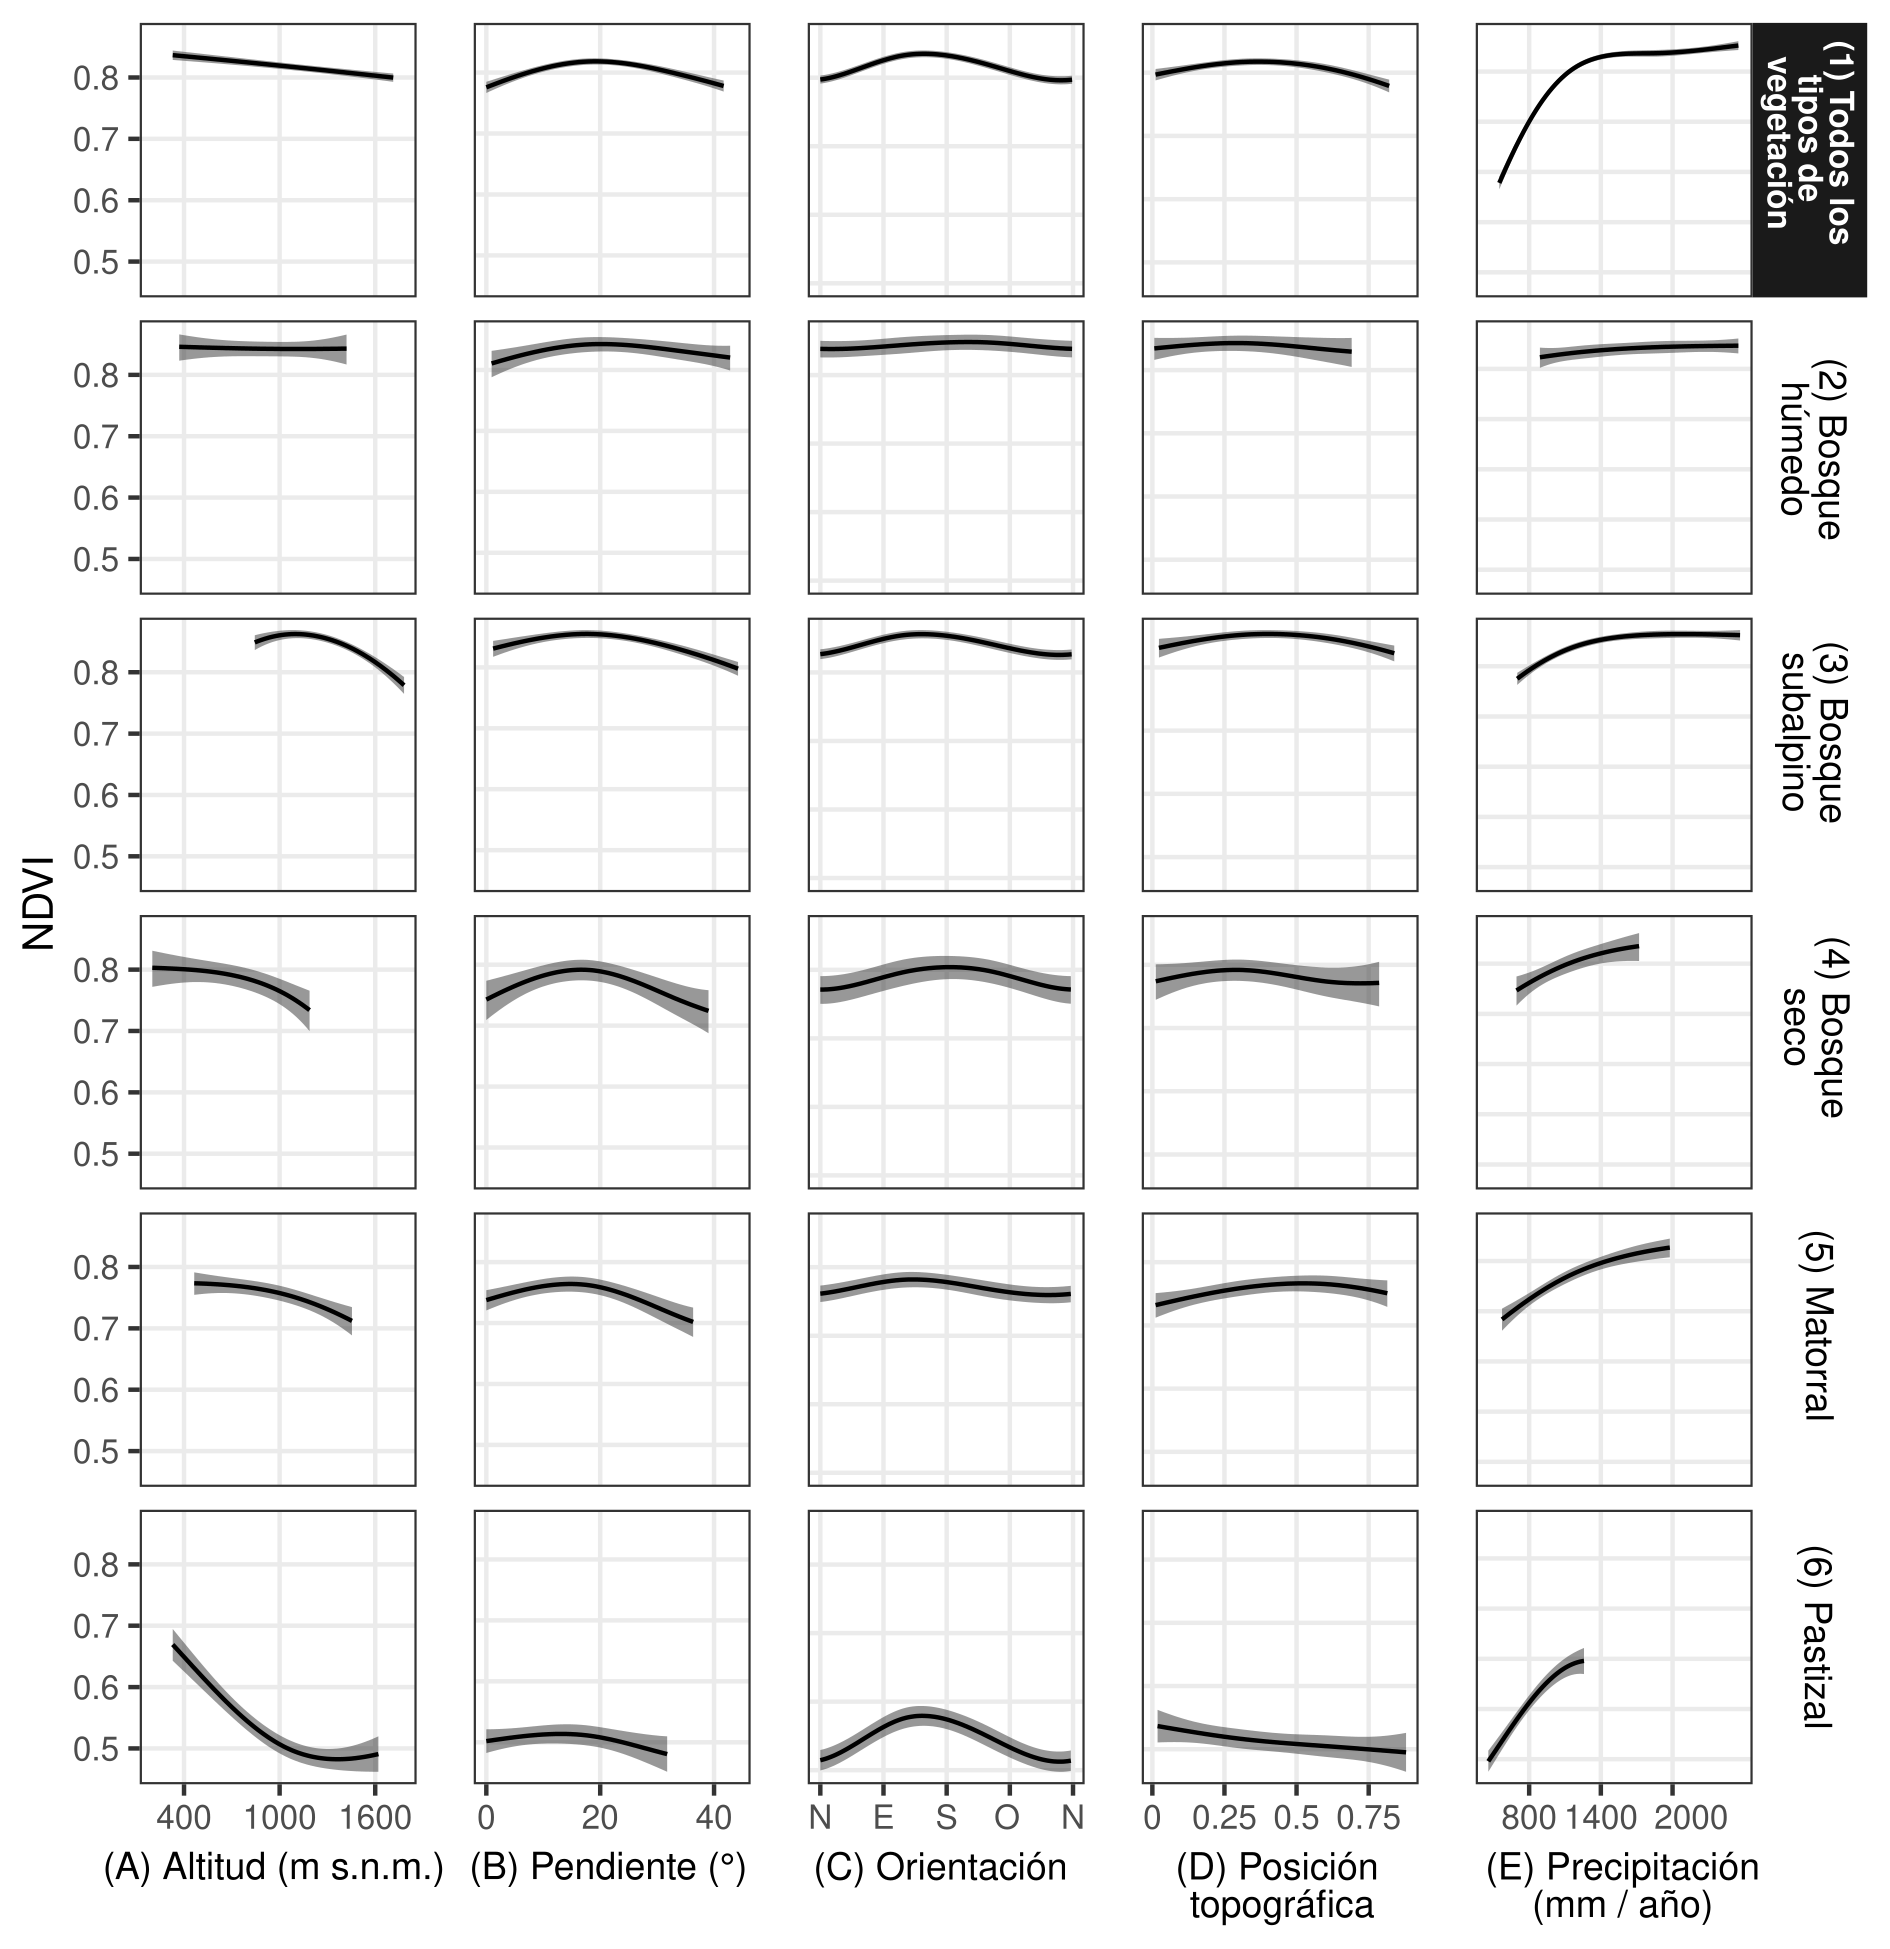
\includegraphics[width=16cm]{figuras/cap3/S07) ndvi_model_predictions.png}
    \caption[NDVI en función de variables ambientales.]{NDVI en función de variables topográficas y precipitación, calculado a lo largo del intervalo de máxima densidad del 98 \% en cada tipo de vegetación. Las líneas muestran la predicción a partir de la estimación de máxima verosimilitud, y las bandas, el intervalo de confianza del 95 \%.} 
    \label{fig:cap3-S07}
\end{figure}

\begin{figure}
    \centering
    \rotatebox[origin=c]{90}{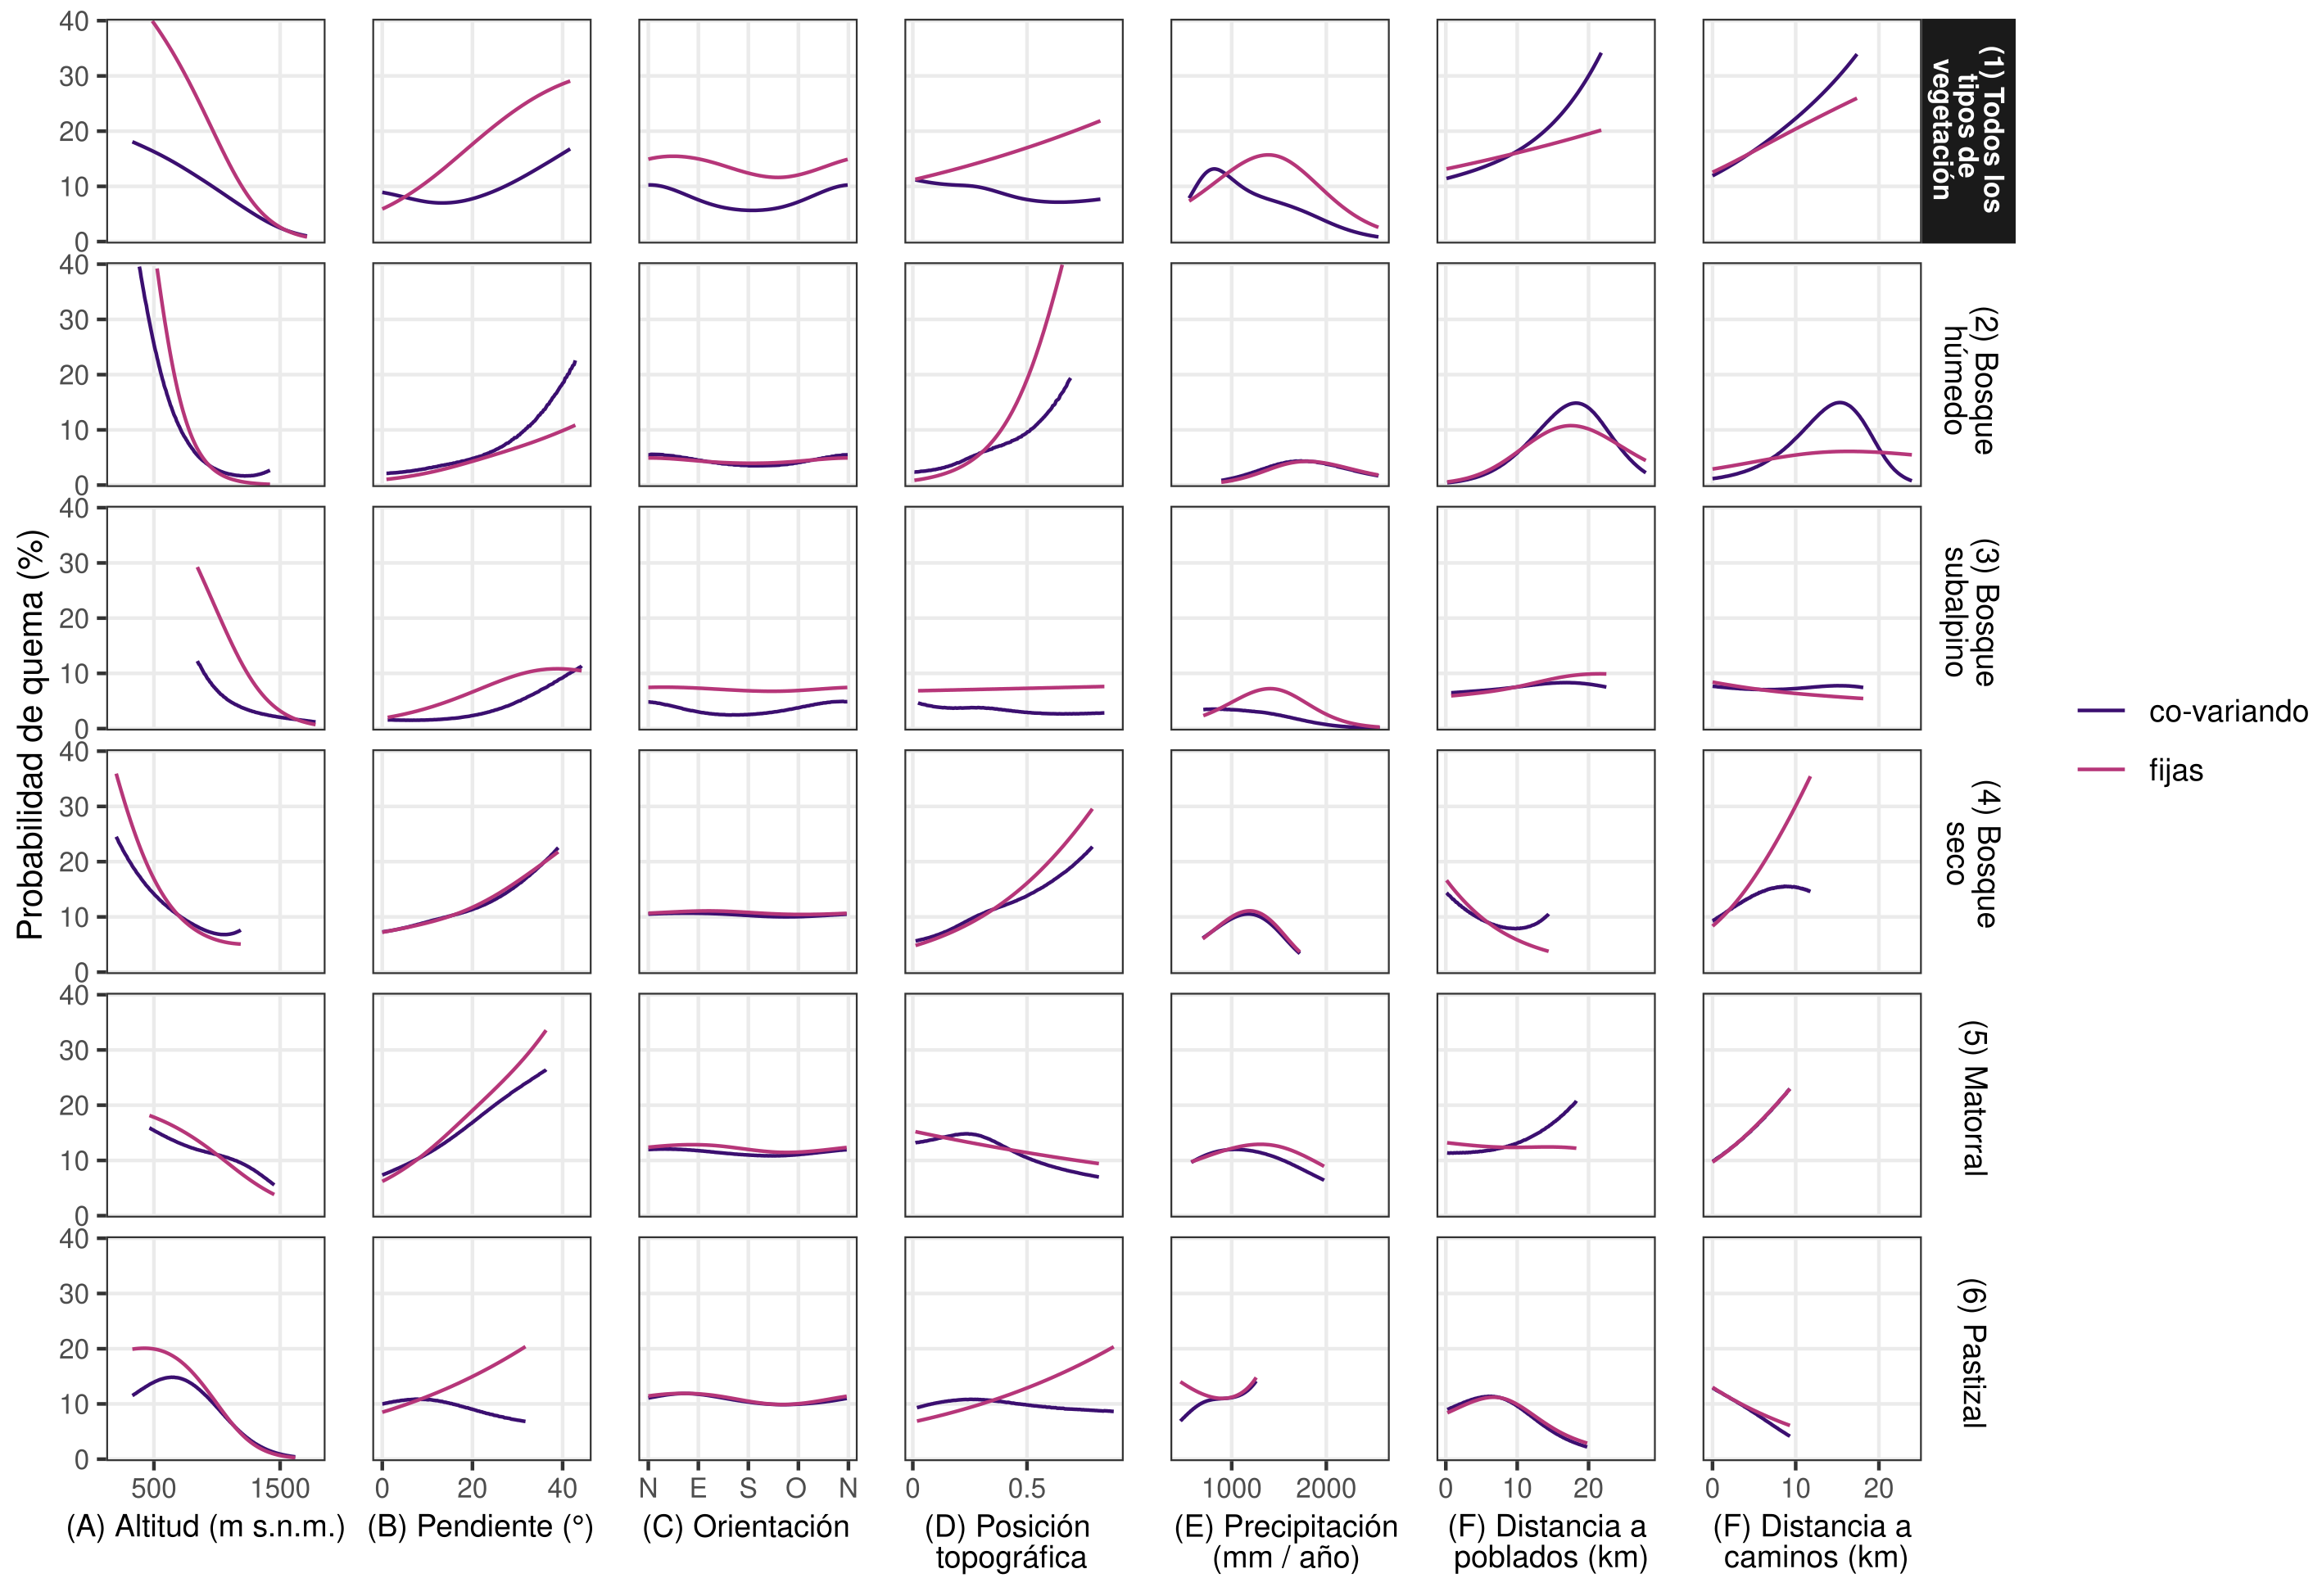
\includegraphics[width=0.95\textheight]{figuras/cap3/S08) burnprob_co-varying_fixed.png}}
    \caption[Probabilidad de quema covariando o fijando predictoras correlacionadas.]{(Leyenda en la página siguiente.)} 
    \label{fig:cap3-S08}
\end{figure}

% leyenda en la página siguiente
\begin{figure}[p]
  \contcaption{(en la página anterior). Probabilidad de quema en función de la topografía, la precipitación y la distancia a poblados y caminos, predicha considerando la covariación entre predictoras o no (predicciones fijas, estrictamente parciales). Las líneas más oscuras muestran las mismas predicciones que las Fig.~\ref{fig:cap3-04} y \ref{fig:cap3-05} del Capítulo~\ref{cap:patrones}.}
\end{figure}

\FloatBarrier

\subsection{Métrica de tamaño de efecto}\label{append:effsize}

Para las variables ambientales y el NDVI (predictoras continuas), el tamaño del efecto se definió como la desviación absoluta media de la curva de predicción no tan parcial, ponderando cada valor de la predictora por su densidad empírica, tanto para calcular la media a lo largo de la curva como para promediar la diferencia absoluta con respecto a la media. En el caso del tipo de vegetación, el cálculo fue similar, pero en lugar de utilizar una curva de predicción utilizamos la probabilidad de quema predicha para todos los tipos de vegetación, ya fuera a partir del modelo de vegetación, o a partir del PDP particionado calculado en base al modelo conjunto (sección~\ref{append:veg-comparison}). Para el modelo de vegetación, los pesos de cada tipo de vegetación se definieron como sus abundancias relativas en el paisaje. Cuando se compararon los tipos de vegetación en condiciones ambientales comunes con el modelo conjunto (PDP particionado), se calculó el tamaño del efecto del tipo de vegetación en cada partición. En ese caso, los pesos se definieron en base a la abundancia relativa de los tipos de vegetación comparados dentro de cada partición del conjunto de datos.

\subsection{Detección de patrones bajo correlación espacial}\label{append:pvalues}

Dado que la correlación espacial conduce a una subestimación de la incertidumbre, en lugar de calcular intervalos de confianza, evaluamos la incertidumbre comparando nuestros resultados con los de conjuntos de datos de incendios aleatorizados que presentaban una correlación similar. Simulamos 500 capas de ocurrencia de incendios, convirtiendo cada incendio observado en un círculo de la misma área y reubicando sus centroides al azar dentro del área quemable, permitiendo que los incendios se solaparan. Estas capas de incendios se rasterizaron y se muestrearon en los mismos 8228 puntos de los que se extrajeron los datos observados. A continuación, todos los análisis realizados con los datos observados se repitieron para cada de quema aleatorizada. Para los efectos de las predictoras continuas, calculamos los valores P a una cola como $1 - \pi$, donde $\pi$ es el percentil correspondiente al efecto observado en la distribución de efectos de los conjuntos de datos aleatorizados. Para las probabilidades de quema por tipo de vegetación, calculamos los valores P a dos colas de la siguiente manera: 

\begin{equation}
    \text{P} = 
    \begin{cases}
        \pi \ 2, & \text{para } \pi < 0.5 \\
        (1-\pi) \ 2 & \text{para } \pi \ge 0.5 
    \end{cases}
\label{eq:p-value}
\end{equation}

Donde $\pi$ es el percentil de la probabilidad de quema observada en la distribución de incendios aleatorios. Además, al graficar predicciones parciales para las predictoras continuas, calculamos los intervalos centrales de colas equiprobables (\textit{equal-tailed intervals}) del 80 \% y el 95 \% de todas las curvas de predicción parcial aleatorizadas (basadas en la estimación de máxima verosimilitud) y evaluamos visualmente en qué medida la curva obtenida con los datos observados se alejaba de esos intervalos.